%%%%%%%%%%%%%%%%%%%%%%%%%%%%%%%%%%%%%%%%%%%%%%%%%%%%%%%%%%%%%%%
%% OXFORD THESIS TEMPLATE

% Use this template to produce a standard thesis that meets the Oxford University requirements for DPhil submission
%
% Originally by Keith A. Gillow (gillow@maths.ox.ac.uk), 1997
% Modified by Sam Evans (sam@samuelevansresearch.org), 2007
% Modified by John McManigle (john@oxfordechoes.com), 2015
%
% This version Copyright (c) 2015-2017 John McManigle
%
% Broad permissions are granted to use, modify, and distribute this software
% as specified in the MIT License included in this distribution's LICENSE file.
%

% I've (John) tried to comment this file extensively, so read through it to see how to use the various options.  Remember
% that in LaTeX, any line starting with a % is NOT executed.  Several places below, you have a choice of which line to use
% out of multiple options (eg draft vs final, for PDF vs for binding, etc.)  When you pick one, add a % to the beginning of
% the lines you don't want.


%%%%% CHOOSE PAGE LAYOUT
% The most common choices should be below.  You can also do other things, like replacing "a4paper" with "letterpaper", etc.

% This one will format for two-sided binding (ie left and right pages have mirror margins; blank pages inserted where needed):
\documentclass[a4paper,twoside]{main}
% This one will format for one-sided binding (ie left margin > right margin; no extra blank pages):
%\documentclass[a4paper]{ociamthesis}
% This one will format for PDF output (ie equal margins, no extra blank pages):
%\documentclass[a4paper,nobind]{ociamthesis} 

%%%%% SELECT YOUR DRAFT OPTIONS
% Three options going on here; use in any combination.  But remember to turn the first two off before
% generating a PDF to send to the printer!

% This adds a "DRAFT" footer to every normal page.  (The first page of each chapter is not a "normal" page.)
\fancyfoot[C]{\emph{DRAFT Printed on \today}}  

% This highlights (in blue) corrections marked with (for words) \mccorrect{blah} or (for whole
% paragraphs) \begin{mccorrection} . . . \end{mccorrection}.  This can be useful for sending a PDF of
% your corrected thesis to your examiners for review.  Turn it off, and the blue disappears.
\correctionstrue


%%%%% BIBLIOGRAPHY SETUP
% Note that your bibliography will require some tweaking depending on your department, preferred format, etc.
% The options included below are just very basic "sciencey" and "humanitiesey" options to get started.
% If you've not used LaTeX before, I recommend reading a little about biblatex/biber and getting started with it.
% If you're already a LaTeX pro and are used to natbib or something, modify as necessary.
% Either way, you'll have to choose and configure an appropriate bibliography format...

% The science-type option: numerical in-text citation with references in order of appearance.
\usepackage[style=numeric-comp, sorting=none, backend=biber, doi=false, isbn=false]{biblatex}
\newcommand*{\bibtitle}{References}

% The humanities-type option: author-year in-text citation with an alphabetical works cited.
%\usepackage[style=authoryear, sorting=nyt, backend=biber, maxcitenames=2, useprefix, doi=false, isbn=false]{biblatex}
%\newcommand*{\bibtitle}{Works Cited}

% This makes the bibliography left-aligned (not 'justified') and slightly smaller font.
\renewcommand*{\bibfont}{\raggedright\small}

% Change this to the name of your .bib file (usually exported from a citation manager like Zotero or EndNote).
\addbibresource{main.bib}


% Uncomment this if you want equation numbers per section (2.3.12), instead of per chapter (2.18):
%\numberwithin{equation}{subsection}



%%%%% THESIS / TITLE PAGE INFORMATION
% Everybody needs to complete the following:
\title{Regulation of the pancreatic K\textsubscript{ATP} channel}
\author{Samuel Usher}
\college{Green Templeton College}

% Master's candidates who require the alternate title page (with candidate number and word count)
% must also un-comment and complete the following three lines:
%\masterssubmissiontrue
%\candidateno{933516}
%\wordcount{28,815}

% Uncomment the following line if your degree also includes exams (eg most masters):
%\renewcommand{\submittedtext}{Submitted in partial completion of the}
% Your full degree name.  (But remember that DPhils aren't "in" anything.  They're just DPhils.)
\degree{Doctor of Philosophy}
% Term and year of submission, or date if your board requires (eg most masters)
\degreedate{Trinity 2021}


%%%%% YOUR OWN PERSONAL MACROS
% This is a good place to dump your own LaTeX macros as they come up.

% To make text superscripts shortcuts
	\renewcommand{\th}{\textsuperscript{th}} % ex: I won 4\th place
	\newcommand{\nd}{\textsuperscript{nd}}
	\renewcommand{\st}{\textsuperscript{st}}
	\newcommand{\rd}{\textsuperscript{rd}}

% To make coloured figure backgrounds and allow for multipanel figures
\usepackage{caption}
\usepackage{subcaption}
\usepackage{mdframed}
\usepackage{lipsum}
\usepackage{xcolor}
\definecolor{bg_figure}{RGB}{239, 235, 233}

\let\originalfigure=\figure
\let\endoriginalfigure=\endfigure

\renewenvironment{figure}[1][]{
  \begin{originalfigure}[#1]
    \begin{mdframed}[linecolor=black!30,backgroundcolor=bg_figure]
}{
    \end{mdframed}
  \end{originalfigure}
}
\DeclareCaptionLabelFormat{bold}{\textbf{#2)}}
\DeclareCaptionSubType[Alph]{figure}
\DeclareCaptionSubType[Alph]{subfigure}

\captionsetup[subfigure]{
	position=top,
	labelfont=bf,
	textfont=small,
	singlelinecheck=off,
	justification=raggedright,
	labelformat=simple
	}

\captionsetup[figure]{
	position=bottom,
	labelfont={bf,sc},
	textfont=small,
	justification=justified,
	labelformat=simple,
	subrefformat=bold
	}

%%%%% THE ACTUAL DOCUMENT STARTS HERE
\begin{document}



%%%%% CHOOSE YOUR LINE SPACING HERE
% This is the official option.  Use it for your submission copy and library copy:
\setlength{\textbaselineskip}{22pt plus2pt}
% This is closer spacing (about 1.5-spaced) that you might prefer for your personal copies:
%\setlength{\textbaselineskip}{18pt plus2pt minus1pt}

% You can set the spacing here for the roman-numbered pages (acknowledgements, table of contents, etc.)
\setlength{\frontmatterbaselineskip}{17pt plus1pt minus1pt}

% Leave this line alone; it gets things started for the real document.
\setlength{\baselineskip}{\textbaselineskip}


%%%%% CHOOSE YOUR SECTION NUMBERING DEPTH HERE
% You have two choices.  First, how far down are sections numbered?  (Below that, they're named but
% don't get numbers.)  Second, what level of section appears in the table of contents?  These don't have
% to match: you can have numbered sections that don't show up in the ToC, or unnumbered sections that
% do.  Throughout, 0 = chapter; 1 = section; 2 = subsection; 3 = subsubsection, 4 = paragraph...

% The level that gets a number:
\setcounter{secnumdepth}{2}
% The level that shows up in the ToC:
\setcounter{tocdepth}{2}


%%%%% ABSTRACT SEPARATE
% This is used to create the separate, one-page abstract that you are required to hand into the Exam
% Schools.  You can comment it out to generate a PDF for printing or whatnot.
\begin{abstractseparate}
	ATP-sensitive potassium (K\ATP{}) channels are present in many tissues, most notably pancreatic islets and cardiac cells, where they couple the metabolic state of a cell to its electrical activity by regulating the flow of K\textsuperscript{} across the membrane in response to the intracellular ATP/ADP ratio.
K\ATP{} channels are an octameric complex, comprised of four inwardly-rectifying potassium channel (Kir) subunits, each of which is associated with a sulphonylurea receptor (SUR) subunit. 
In pancreatic islets, K\ATP{} channels are formed by Kir6.2 and SUR1.

The physiological regulation of K\ATP{} activity by the ATP/ADP ratio is the summed contribution of activation by Mg-nucleotides binding to SUR1, and inhibition by nucleotides binding to Kir6.2.
Mutations in either Kir6.2 and SUR1 which lead to diseases of insulin secretion are frequently observed to disrupt the nucleotide regulation of the channel.
 % Create an abstract.tex file in the 'text' folder for your abstract.
\end{abstractseparate}


% JEM: Pages are roman numbered from here, though page numbers are invisible until ToC.  This is in
% keeping with most typesetting conventions.
\begin{romanpages}

% Title page is created here
\maketitle

%%%%% DEDICATION -- If you'd like one, un-comment the following.
%\begin{dedication}
%This thesis is dedicated to\\
%someone\\
%for some special reason\\
%\end{dedication}

%%%%% ACKNOWLEDGEMENTS -- Nothing to do here except comment out if you don't want it.
\begin{acknowledgements}
 	First of all, thank you Fran for your endless well of knowledge, and your support and encouragement throughout my time in your lab.
Your enthusiasm for science will continue to inspire me, and I will always be grateful for your patience.
Thank you Mike, for taking on a graduate student who had never patched a cell before and infusing me with your love for ion channels.
I couldn't have asked for a better friend and colleague.

Thank you to the Ashcroft lab, past and present, for your companionship, expertise, and hard work - Raul, Idoia, Natascia, Lizzie, Gregor, Will.
It has been a privilege to work and learn alongside you.
Thank you to the other members of the ion channel journal club for putting up with my ramblings and contributing some of your own.
Harvey, Brad, Max - it's been a pleasure falling back in love with Oxford with you guys.

Thank you Meg for your constant support and for being a shoulder to lean on whenever I have needed it.
Finally, thank you to my family - Mum, Dad, I will never be able to fully express my gratitude for everything you have done to get me here.
\end{acknowledgements}

%%%%% ABSTRACT -- Nothing to do here except comment out if you don't want it.
\begin{abstract}
	ATP-sensitive potassium (K\ATP{}) channels are present in many tissues, most notably pancreatic islets and cardiac cells, where they couple the metabolic state of a cell to its electrical activity by regulating the flow of K\textsuperscript{} across the membrane in response to the intracellular ATP/ADP ratio.
K\ATP{} channels are an octameric complex, comprised of four inwardly-rectifying potassium channel (Kir) subunits, each of which is associated with a sulphonylurea receptor (SUR) subunit. 
In pancreatic islets, K\ATP{} channels are formed by Kir6.2 and SUR1.

The physiological regulation of K\ATP{} activity by the ATP/ADP ratio is the summed contribution of activation by Mg-nucleotides binding to SUR1, and inhibition by nucleotides binding to Kir6.2.
Mutations in either Kir6.2 and SUR1 which lead to diseases of insulin secretion are frequently observed to disrupt the nucleotide regulation of the channel.

\end{abstract}

%%%%% MINI TABLES
% This lays the groundwork for per-chapter, mini tables of contents.  Comment the following line
% (and remove \minitoc from the chapter files) if you don't want this.  Un-comment either of the
% next two lines if you want a per-chapter list of figures or tables.
\dominitoc % include a mini table of contents
%\dominilof  % include a mini list of figures
%\dominilot  % include a mini list of tables

% This aligns the bottom of the text of each page.  It generally makes things look better.
\flushbottom

% This is where the whole-document ToC appears:
\tableofcontents

\listoffigures
	\mtcaddchapter
% \mtcaddchapter is needed when adding a non-chapter (but chapter-like) entity to avoid confusing minitoc

% Uncomment to generate a list of tables:
%\listoftables
%	\mtcaddchapter

%%%%% LIST OF ABBREVIATIONS
% This example includes a list of abbreviations.  Look at text/abbreviations.tex to see how that file is
% formatted.  The template can handle any kind of list though, so this might be a good place for a
% glossary, etc.
\graphicspath{{figures/appendix/}}

\begin{mclistof}{List of Abbreviations}{3.2cm}

\item[ABC] ATP-binding cassette

\item[ADP] Adenosine diphosphate

\item[ATP] Adenosine triphosphate

\item[ANAP] L-3-(6-acetylnaphthalen-2-ylamino)-2-aminopropionic acid

\item[CFTR] Cystic fibrosis transmembrane conductance regulator

\item[Cryo-EM] Cryo-electron microscopy

\item[EC\textsubscript{50}] Half maximal effective concentration

\item[ER] Endoplasmic reticulum

\item[FRET] F\"{o}rster resonance energy transfer

\item[GFP] Green fluorescent protein

\item[HA] Human influenza hemagglutinin

\item[HEK293T] Human embryonic kidney 293 cells containing the SV40 T-antigen

\item[IC\textsubscript{50}] Half maximal inhibitory concentration

\item[K\ATP{} channel] ATP-sensitive potassium channel

\item[Kir] Inward rectifier potassium channel

\item[L0] Loop zero

\item[LOO-CV] Leave-one-out cross-validation

\item[mO] mOrange fluorescent protein

\item[MWC] Monod-Wyman-Changeaux

\item[NBD] Nucleotide binding domain

\item[PCF] Patch-clamp fluorometry

\item[PDB] Protein data bank

\item[PIP\textsubscript{2}] Phosphatidylinositol 4,5-bisphosphate

\item[$P_O$] Open probability

\item[SUR] Sulphonylurea receptor

\item[TEA\textsuperscript{+}] Triethylammonium ion

\item[TMD] Transmembrane domain

\item[TNP-ADP] Trinitrophenyl adenosine diphosphate

\item[TNP-ATP] Trinitrophenyl adenosine triphosphate

\item[UAA] Unnatural amino acid

\item[WT] Wild-type

\end{mclistof}

\begin{figure}[h]
	\centering
	\begin{subfigure}[t]{0.45\textwidth}
		\caption{}\label{ch0fig:kir_constructs}
		\centering
		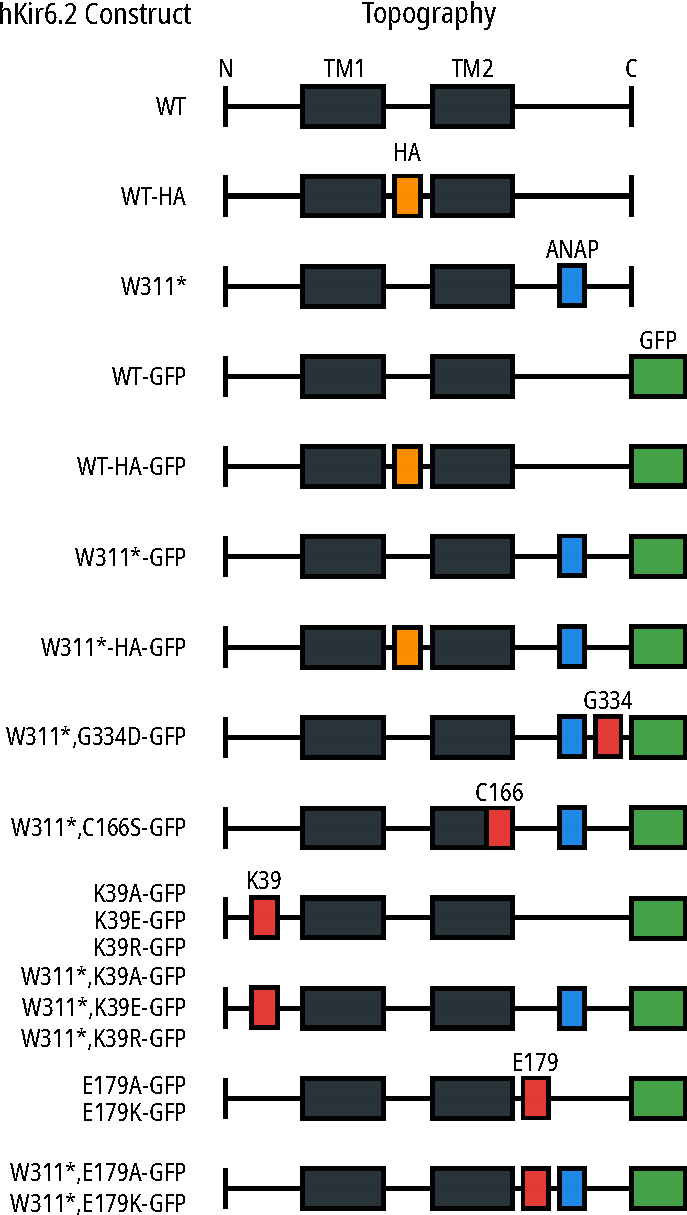
\includegraphics[width=\textwidth]{kir_constructs.pdf}
	\end{subfigure}
	\hfill
	\begin{subfigure}[t]{0.45\textwidth}
		\caption{}\label{ch0fig:sur_constructs}
		\centering
		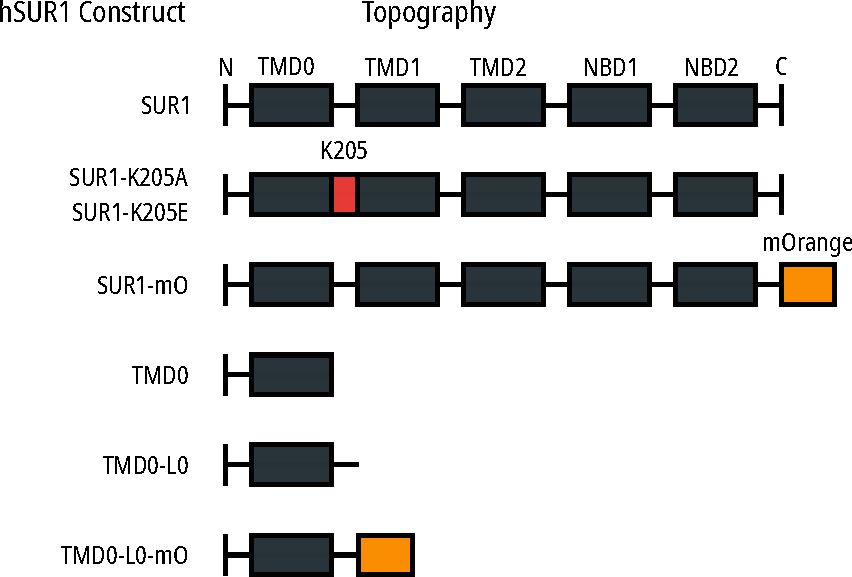
\includegraphics[width=\textwidth]{sur_constructs.pdf}
	\end{subfigure}
	\caption[hKir6.2 and hSUR1 constructs and their abbreviations]{
	}\label{ch0fig:constructs}
\end{figure}

% The Roman pages, like the Roman Empire, must come to its inevitable close.
\end{romanpages}


%%%%% CHAPTERS
% Add or remove any chapters you'd like here, by file name (excluding '.tex'):
\flushbottom
\chapter{\label{ch:1-intro}Introduction} 

\graphicspath{{figures/ch1/}}

\minitoc

\section{General introduction}

\section{Pancreatic islets and the \textgreek{b}-cell}

Pancreatic islets are endocrine cells which are responsible for maintaining glucose homeostasis.
There are roughly one million islets in a human pancreas, constituting 1-2\% of the total pancreatic mass.
Islets consist of three principal cell types; insulin secreting \textgreek{b}-cells, glucagon secreting \textgreek{a}-cells and somatostatin secreting \textgreek{D}-cells.
Islets respond to increases in blood glucose by releasing insulin, which acts on peripheral tissues to increase glucose uptake and reduce blood glucose levels.
Conversely, decreases in blood glucose leads to the release of glucagon, which acts on those tissues to stimulate glucose production and increase blood glucose.

\section{Architecture of the pancreatic K\ATP{} channel}

ATP-sensitive potassium (K\ATP{}) channels are present in many tissues, where they couple the metabolic state of a cell to its electrical activity by regulating the flow of K\textsuperscript{+} across the membrane.
K\ATP{} channels are an octameric complex, comprised of four inwardly-rectifying potassium channel subunits (Kir6.1 or Kir6.2), each of which is associated with a sulphonylurea receptor subunit (SUR1, SUR2A or SUR2B).
In pancreatic \textgreek{b}-cells, the K\ATP{} channel isoform is composed of Kir6.2 and SUR1.
Together, Kir6.2 and SUR1 form a complex nearly a megadalton in size and over 15 nanometres across (Figure \ref{ch1fig:katp_cartoon}, \ref{ch1fig:sur_topdown}).

Inwardly-rectifying potassium channels are so named because they allow K\textsuperscript{+} to flow more easily into the cell than out of it (Figure \ref{ch1fig:rectification}).
This phenomenon is a consequence of voltage-dependent pore blockade by intracellular divalent cations (especially Mg\textsuperscript{2+}) and polyamines.
At depolarising membrane potentials, blockers are driven into the pore and K\textsuperscript{+} current is blocked, while at hyperpolarising potentials the blockers and cleared and K\textsuperscript{+} current can flow.
Strongly rectifying Kir channels display drastically reduced conductance at potentials more positive than the K\textsuperscript{+} reversal potential.
In contrast, Kir6.2 is a weak rectifier, and allows substantial current to flow at more positive potentials.

In addition to voltage, Kir6.2 is regulated by two endogenous ligands; 
phosphatidylinositol 4,5-bisphosphate (PIP\textsubscript{2}) and adenine nucleotides (Figure \ref{ch1fig:kir_struct}).
The binding of adenine nucleotides to Kir6.2 leads to closure of the channel pore, while the binding of PIP\textsubscript{2} promotes the opening of the pore (Figure \ref{ch1fig:shyng_trace}).
Activation by PIP\textsubscript{2} is a mechanism common to the whole Kir family, wherease inhibition by nucleotides is unique to the Kir6 subfamily.

\begin{figure}[h]
	\centering
	\begin{subfigure}[t]{0.5\textwidth}
		\caption{}\label{ch1fig:rectification}
		\centering
		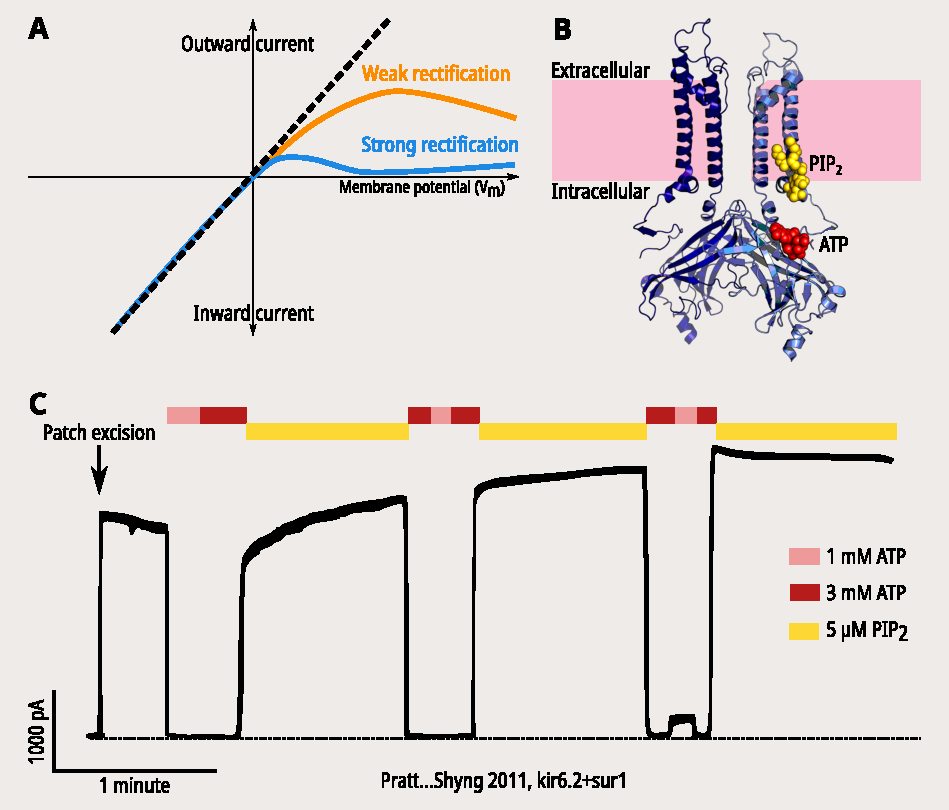
\includegraphics[width=\textwidth]{rectification.pdf}
	\end{subfigure}
	\hfill
	\begin{subfigure}[t]{0.4\textwidth}
		\caption{}\label{ch1fig:kir_struct}
		\centering
		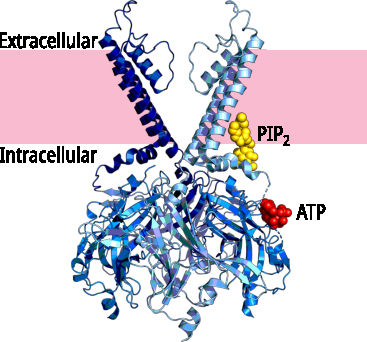
\includegraphics[width=\textwidth]{kir_structure.pdf}
	\end{subfigure}
	\vfill
	\begin{subfigure}[t]{0.9\textwidth}
		\caption{}\label{ch1fig:shyng_trace}
		\centering
		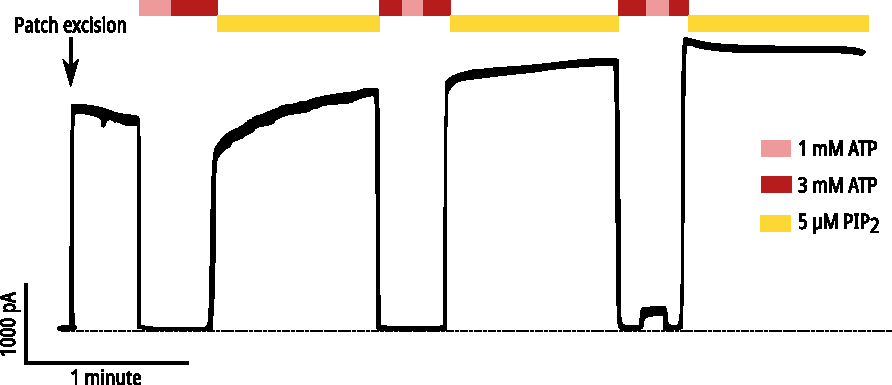
\includegraphics[width=\textwidth]{shyng_atp_pip_trace.pdf}
	\end{subfigure}
	\caption[Structure of Kir6.2]{
		\subref{ch1fig:rectification} Current-voltage plot demonstrating inward rectification of Kir channels.
		Here, the reversal potential of potassium (\textit{E\textsubscript{K}}) is set to zero, i.e. there is an equal concentration of K\textsuperscript{+} on each side of the membrane.
		Weak rectifiers such as Kir6.2 exhibit only a weak voltage dependent decline in conductance (visualised as a departure from the dashed line of an ideal conductor).
		(Kind of adapted from Handbook of Ion Channels).
		\subref{ch1fig:kir_struct} Cryo-EM structure of Kir6.2 (PDB \#6BAA) captured with ATP bound (red) and with the proposed binding position of PIP\textsubscript{2} visualised by alignment of the channel with the X-ray structure of Kir2.2 solved in compex with a short-chain dioctanoyl (diC8) PIP\textsubscript{2} (PDB \#6C3I).
		The plasma membrane is shown in pink.
		(Kind of adapted from Mike's JGP review).
		\subref{ch1fig:shyng_trace} Macroscopic currents from Kir6.2 channels coexpressed with SUR1 in excised patches from cultured cells, adapted from (Pratt/Shyng, 2011).
		Perfusion of ATP or PIP\textsubscript{2} is indicated by coloured bars, and demonstrates the contrasting effects of these two ligands on channel activity.
	}
	\label{ch1fig:kir_breakdown}
\end{figure}

SUR1 is a member of the ATP-binding cassette (ABC) family of transporters.
While other ABC proteins transport substrate across the membrane, SUR1 does not appear to do so; instead it acts to modulate the function of its associated ion channel.
The cystic fibrosis transmembrane conductance regulator (CFTR) is another member of the ABC family, and is an ion channel in its own right, capable of conducting chloride across the membrane.
Like other ABC proteins, SUR1 contains two sets of transmembrane domains (TMD1 and TMD2) and two cytosolic nucleotide binding domains (NBD1 and NBD2).
Unique to SUR is the presence of an additional transmembrane domain (TMD0) N-terminal to the core of the protein, and this domain forms the primary contact between SUR1 and Kir6.2.

The NBDs of ABC transporters are highly conserved, and consist of two subdomains: a larger RecA-like subdomain found in other P-loop ATPases, and a smaller \textgreek{a}-helical subdomain which is unique to ABC transporters.
There are three key structural motifs present in these subdomains: the RecA-like subdomain contains the Walker A (W\textsubscript{A}) and B (W\textsubscript{B}) motifs, while the \textgreek{a}-helical subdomain contains the ABC signature motif (typically LSGGQ).

The two domains come together to form an antiparallel dimer with two nucleotide binding sites (NBS1 and NBS2) at the interface, such that NBS1 is formed from the W\textsubscript{A} and W\textsubscript{B} motifs of NBD1 and the signature motif from NBD2, whereas NBS2 is formed from the W\textsubscript{A} and W\textsubscript{B} motifs of NBD2 and the signature motif from NBD1.
NBS2, also known as the consensus site as it is more similar in sequence to other ABC family members, is catalytically competent and able to hydrolyse ATP.
In contrast, NBS1 is the degenerate site, with a less conserved sequence and an inability to catalyse hydrolysis of ATP.

\begin{figure}[h]
	\centering
	\begin{subfigure}[t]{0.4\textwidth}
		\caption{}\label{ch1fig:sur_struct}
		\centering
		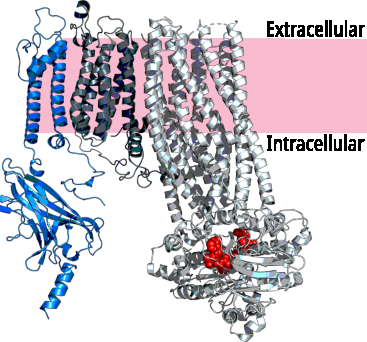
\includegraphics[width=\textwidth]{sur_structure.pdf}
	\end{subfigure}
	\hfill
	\begin{subfigure}[t]{0.5\textwidth}
		\caption{}\label{ch1fig:nbd_struct}
		\centering
		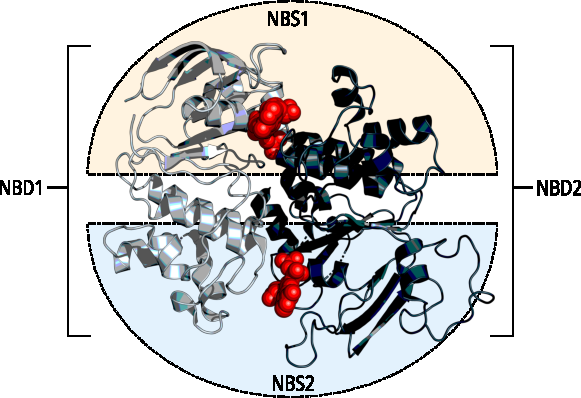
\includegraphics[width=\textwidth]{nbd_structure.pdf}
	\end{subfigure}
	\caption[Structure of SUR1]{
		\subref{ch1fig:sur_struct} Cryo-EM structure of SUR1 captured with a nucleotide (shown in red) bound at each NBS (PDB \#6C3P).
		A single SUR1 subunit is shown, with TMD1 and TMD2 in white and TMD0 in grey.
		A single Kir6.2 subunit is also shown in blue to show the interface between subunits.
		The plasma membrane is displayed in pink.
		\subref{ch1fig:nbd_struct} Top-down view of the NBDs from the same cryo-EM structure.
		NBD1 is on the left in white, NBD2 is on the right in grey, and the two NBSs are higlighted; NBS1 in orange and NBS2 in blue.
		Adapted from Mikes JGP review.
	}
\end{figure}

\section{Ligand-independent regulation of the pancreatic K\ATP{} channel}

\subsection{Assembly and trafficking}

Biogenesis of K\ATP{} channels occurs in the endoplasmic reticulum (ER), and is an important checkpoint in determining surface expression and channel stoichiometry \cite{zerangue_new_1999-1, martin_pharmacological_2013}.
The precise nature of the events which occur between subunit translation and insertion of octameric K\ATP{} into the cell membrane are not fully mapped out, but studies have highlighted some important quality control steps in this process which regulate K\ATP{} channel expression.
When Kir6.2 or SUR1 are expressed alone in heterologous systems, they are retained in the ER \cite{zerangue_new_1999-1}.
This mechanism is achieved through the exposure of a three amino acid ER-retention motif (RKR) in the cytoplasmic domains of both Kir6.2 and SUR1.
Only upon complete assembly of the channel complex are the RKR motifs masked, allowing forward trafficking of K\ATP{} to the cell surface.
Deletion of the RKR motif \cite{tucker_truncation_1997}, or mutation of the motif to AAA \cite{zerangue_new_1999-1}, results in unregulated surface expression of individual subunits and/or partially assembled channel complexes.
Addition of a GFP label to the C-terminus of Kir6.2 is also sufficient to allow trafficking of subunits to the cell surface in the absence of SUR1 \cite{john_sulphonylurea_1998-1}.

In addition to the RKR motif, there are two N-linked glycosylation sites on SUR1 (N10 and N1050) which are required for cell surface expression \cite{conti_membrane_2002}.
Mutation of these sites to glutamines results in retention in the ER and drastically reduced expression of K\ATP{} on the cell surface.
This mechanism is thought to be separate to that for the ER-retention motif, as mutation of RKR to AAA is not sufficient to drive surface expression of the glycosylation mutants \cite{conti_membrane_2002}.

A putatitive third site of trafficking regulation is in the C-terminus of SUR1.
Mutation or deletion of a dileucine motif 16 amino acids distal to the C-terminal of SUR1 results in reduced surface expression of K\ATP{} channels in COSm6 cells \cite{sharma_c_1999}.
This reduction in expression is not rescued by C-terminal truncation of Kir6.2, indicating that this result is not due to masking of the RKR retention motif.
The dileucines are therefore suggested to promote forward trafficking of assembled channel complexes to the cell membrane \cite{sharma_c_1999}.
Expression of K\ATP{} channels expressed in \textit{Xenopus} oocytes is also dramatically reduced by truncation of the C-terminal 42 amino acids of SUR1 \cite{vedovato_role_2018}.
However, longer deletions of the SUR1 C-terminus did not reduce surface expression of channels in HEK293 cells \cite{giblin_cytoplasmic_2002}, and other modifications of the SUR1 C-terminus do not exhibit effects on surface expression \cite{schwappach_molecular_2000}.
In fact, a splice variant of SUR1 missing the entirety of the NBD2 domain (truncated at residue 1355) was found to successfully traffic to the membrane of insulin-secreting \textgreek{b}-cell line MIN6 cells \cite{sakura_altered_1999-1}.
The precise role of the dileucine motif remains unclear, and is potentially confounded by the use of expression system \cite{giblin_cytoplasmic_2002, martin_pharmacological_2013}

Failure of the channel complex to pass these three checkpoints results in ER-associated degradation (ERAD), a common pathway shared by most membrane and secretory proteins \cite{bonifacino_ubiquitin_1998, yan_role_2005}.
Both SUR1 and Kir6.2 are substrates for polyubiquitination, both when heterologously expressed and in INS-1 cells \cite{yan_role_2005}.
Application of proteasome inhibitors both reduces the rate of degradation for Kir6.2 and SUR1, and increases the surface expression of K\ATP{} channels by increasing their biogenesis efficiency \cite{yan_role_2005}.

The surface expression of K\ATP{} channels is therefore controlled by a variety of different quality control mechanism to ensure that only correctly assembled octameric channel complexes reach the cell membrane.
Mutations which lead to defects in assembly and trafficking are therefore a common cause of congenital hyperinsulinemia (HI).
These mutations are found throughout both Kir6.2 and SUR1, although they are more commonly found in SUR1 \cite{martin_pharmacological_2013}.

Interestingly, sulphonylureas are able to act as pharmacological chaperones and rescue surface expression of several mutations which would otherwise not traffic to the cell surface \cite{yan_sulfonylureas_2004, yan_sulfonylureas_2006, yan_congenital_2007, yan_congenital_2007-1, martin_pharmacological_2016}.
Sulphonylureas bind directly to the channel during biogenesis, as mutation of residues in SUR1 which are critical for sulphonylurea binding abolished or reduced the effectiveness of expression rescue \cite{yan_sulfonylureas_2006}.
Pharmacological chaperoning requires full assembly of the channel complex, as the presence of Kir6.2 was required to rescue expression of trafficking mutants even when the SUR1 RKR motif was mutated to AAA \cite{yan_sulfonylureas_2006}.
In addition, reducing the temperature at which cells are cultured can rescue some trafficking defects \cite{yang_low_2005}.

\begin{figure}[h]
	\centering
	\begin{subfigure}[t]{0.9\textwidth}
		\caption{}\label{ch1fig:katp_cartoon}
		\centering
		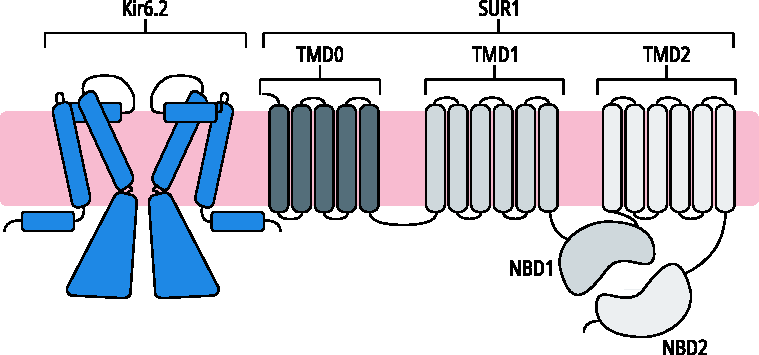
\includegraphics[width=\textwidth]{katp_cartoon.pdf}
	\end{subfigure}
	\vfill
	\begin{subfigure}[t]{0.45\textwidth}
		\caption{}\label{ch1fig:sur_topdown}
		\centering
		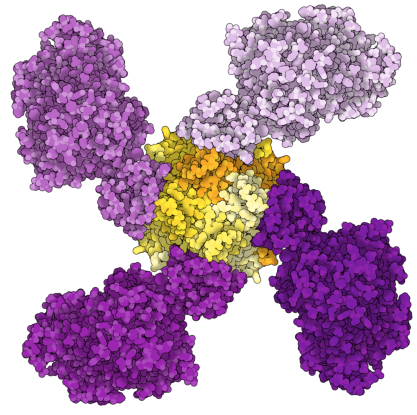
\includegraphics[width=\textwidth]{sur_topdown_propellor.pdf}
	\end{subfigure}
	\hfill
	\begin{subfigure}[t]{0.45\textwidth}
		\caption{}\label{ch1fig:sur_ctd}
		\centering
		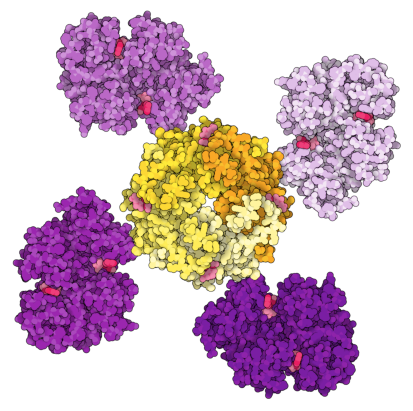
\includegraphics[width=\textwidth]{sur_topdown_ctd_propellor.pdf}
	\end{subfigure}
	\caption[K\ATP{} architecture and nucleotide regulation]{
		\subref{ch1fig:katp_cartoon} Membrane topology of the K\ATP{} channel shown with two Kir6.2 subunits and one SUR1 subunit.
		\subref{ch1fig:sur_topdown} Top-down view of a cryo-EM structure of the K\ATP{} channel (PDB \# 6C3P) solved with nucleotides bound at each of the three canonical binding sites.
		Each SUR1 subunit is shown in a shade of purple, and each Kir6.2 subunit is shown in a shade of orange.
		\subref{ch1fig:sur_ctd} The same view of the structure shown to the left, but with the transmembrane domains removed to reveal the cytoplasmic domains of each subunit only.
		The nucleotides bound to the channel are shown in red.
	}
\end{figure}

\subsection{Regulation of intrinsic gating}

In the absence of nucleotides, K\ATP{} channels are spontaneously active.
This can be seen at a macroscopic level in excised patches.
Upon excision of a patch from a cell membrane containing K\ATP{} channels, the magnitude of current dramatically increases when voltage is applied (Figure \ref{ch1fig:shyng_trace}), reflecting the relief from inhibition of cytoplasmic nucleotides.
While this macroscopic time course is smooth and graded, it consists of hundreds or thousands of individual channels which exhibit binary behaviour; switching between a nonconducting closed state and a conducting open state \ref{hille_ion_2001}.
The summed activity of these individual channels constitutes the large currents observed in macroscopic excised patches.

Single K\ATP{} channels exhibit bursts of brief openings, separated by long interburst closures \cite{alekseev_ligand-insensitive_1998, babenko_two_1999, li_open_2002, proks_modeling_2009}.
Thus, the open probability ($P_O$) of the channel is determined both by the kinetics of the burst (open and closed durations within a burst) and the duration of the long interburst closures.
The intrinsic gating of K\ATP{} can therefore be separated into two separate 'gating' processes; fast (responsible for intraburst closures) and slow (responsible for interburst closures).
While it is helpful to distinguish between fast and slow gating processes to characterise channel regulation, doing so does not require the existence of separate structural gates \cite{proks_modeling_2009, hille_ion_2001}.

Gating is a property intrinsic to Kir6.2, which is able to open and close in the absence of SUR1 \cite{tucker_truncation_1997, enkvetchakul_kinetic_2000-1} (Figure \ref{ch1fig:singles_sur}); albeit with very different kinetic properties which will be discussed later.
The open and intraburst closed time of single channels is dependent on the electrochemical gradient across the cell membrane, otherwise called the K\textsuperscript{+} driving force \cite{benz_characterization_1998}.
As the name implies, the electrochemical gradient depends on two things: the voltage across the membrane, and the K\textsuperscript{+} concentration gradient.
Increasing hyperpolarisation decreases the amount of time channels remain in the open state and increases the amount of time channels remain in the closed state within bursts \cite{alekseev_burst_1997, trapp_molecular_1998-1}.
This is a characteristic feature shared by other inwardly-rectifying K\textsuperscript{+} channels \cite{sakmann_voltage-dependent_1984, alekseev_burst_1997}.
In addition, altering the  K\textsuperscript{+} gradient across the membrane by changing the K\textsuperscript{+} concentration in the pipette or bath solution has the same effect on fast gating kinetics \cite{zilberter_gating_1988, benz_characterization_1998}.
As the driving force for K\textsuperscript{+} increases, the open lifetime of the K\ATP{} channel decreases.
This is in contrast to other K\textsuperscript{+} channels such as K\textsubscript{V}2.1, which exhibits the opposite relationship \cite{chapman_allosteric_2006}.

There are a number of domains within Kir6.2 that regulate the intrinsic gating of the channel.
Firstly, the P-loop is a conserved feature across K\textsuperscript{+} channels (amongst others) \cite{kuang_structure_2015}.
In Kir channels, the P-loop connects the two transmembrane domains, and dips into the plasma membrane to form the K\textsuperscript{+} selectivity filter.
While the P-loop is broadly conserved between Kir family members, there are key residues which differ.
Notably, the K\textsuperscript{+} selectivity filter signature sequence (TxGYG) is identical across all other Kir subtypes (TIGYG), but in Kir6.2 the tyrosine is replaced by a phenylalanine at position 133 (TIGFG), a feature shared only by eag-like K\textsuperscript{+} channels \cite{heginbotham_mutations_1994}.
Another particularly interesting residue is V127, which is unique to Kir6.1 and Kir6.2 within the Kir family - all other Kir channels posess a threonine at this location \cite{proks_mutations_2001}.

\citeauthor{proks_mutations_2001} investigated a range of substitutions at these two residues.
Mutation of V127 to the conserved threonine (V127T) dramatically increases the open time of K\ATP{}, while also increasing the intraburst closed time.
There is also some suggestion of an additional open state existing in this mutant construct, evidenced by the appearance of a second peak in the open time histograms.
Mutation of F133 to the conserved tyrosine (F133Y) did not produce expression of functional channels; however combining the two mutations (V127T,F133Y) resulted in functional channels with a further increase in the open time when compared to the single mutant V127T.
In addition, substitutions at other residues in the P-loop of Kir6.2 leads to a range of effects on the intraburst kinetics of K\ATP{}.
Crucially, none of the substitutions affected the slow gating of the channel; i.e. burst duration and interburst closed times remained similar despite the varied alterations in the intraburst kinetics.
\citeauthor{proks_mutations_2001} concluded that the P-loop is instrumental in regulating the fast gating of K\ATP{}, and suggested that the lack of correlation between perturbations of inter- and intra-burst kinetics is evidence for independence between the fast and slow gating processes.
(I haven't mentioned the correlated decrease in conductance associated with these mutations - need to think more about how this ties in with the regulation of open time by driving force).

Other domains of Kir6.2 are involved in the regulation of slow gating.
The cytosolic end of the second transmembrane domain of Kir6.2 has been implicated in regulation of K\ATP{} slow gating by a number of mutational studies \cite{shyng_control_1997, tucker_molecular_1998, trapp_molecular_1998-1, loussouarn_structure_2000}.
Substitution of C166 with a more bulky or hydrophobic residue dramatically reduces the frequency of the channel entering the long, closed interburst state, and increases the open time of the channel in the bursts \cite{trapp_molecular_1998-1}.
However, no effect is seen on the length of the intraburst closed times, which is additional evidence for the independence of the fast and slow gating processes.
Substitutions at N160 \cite{shyng_control_1997}, L164 \cite{tammaro_kir62_2008}, I167 \cite{tucker_molecular_1998}, and T171 \cite{tucker_molecular_1998, drain_katp_1998} also increase channel open time and decrease the rate of entry into the interburst closed state, further implicating this region of Kir6.2 in modulating the slow gating of K\ATP{}.

The slide-helix of Kir6.2 is the interface between the transmembrane domain and the cytoplasmic domain, and mutations in this region result in changes in the single channel kinetics and $P_O$ of K\ATP{} \cite{proks_molecular_2004, koster_dend_2008, mannikko_interaction_2010, li_decomposition_2013,cooper_conserved_2017}.
Mutations examined at the single channel level show changes in burst duration \cite{proks_molecular_2004, koster_dend_2008, mannikko_interaction_2010} but unaltered intraburst kinetics.
Interpretation of the mechanism underlying these single channel kinetics alterations is complicated by the proximity of this region of Kir6.2 to the putative PIP\textsubscript{2} binding site \cite{pipatpolkai_evaluating_2020}.
Perturbations of this region could be affecting intrinsic gating directly, or indirectly by altering PIP\textsubscript{2} regulation, both of which would lead to changes in slow gating.

While Kir6.2 is able to gate intrinsically when expressed alone, coassembly with SUR1 alters the intrinsic gating of the channel in a number of ways.
Compared to the single channel kinetics of Kir6.2\textgreek{D}C or Kir6.2-GFP alone, coexpression of Kir6.2 with SUR1 increases the open time of the channel within the bursts, and increases their duration, while the intraburst closed times are unaffected \cite{trapp_molecular_1998-1, john_sulphonylurea_1998-1, chan_n-terminal_2003-1}.
This suggests that interactions of SUR1 with Kir6.2 serve to regulate the slow gating of the channel, rather than the fast gating.
The mechanisms by which SUR1 regulates intrinsic gating of the K\ATP{} channel are complex and not yet fully understood.
Structurally, the primary contacts between the two subunits are formed between the N-terminus and first transmembrane domain of Kir6.2 and TMD0 and L0 of SUR1 (Figure \ref{ch1fig:sur_struct}) \cite{martin_anti-diabetic_2017, lee_molecular_2017-1, li_structure_2017-1}.
The contributions of the interactions of these regions have been studied in a variety of ways.

\begin{figure}[h]
	\centering
	\begin{subfigure}[t]{0.45\textwidth}
		\caption{}\label{ch1fig:singles_sur}
		\centering
		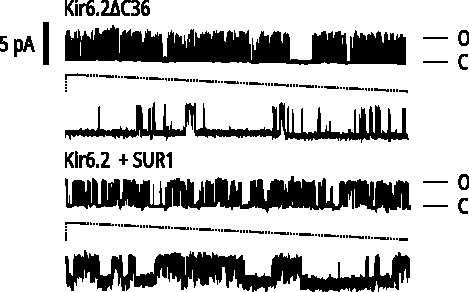
\includegraphics[width=\textwidth]{single_traces_sur.pdf}
	\end{subfigure}
	\hfill
	\begin{subfigure}[t]{0.45\textwidth}
		\caption{}\label{ch1fig:singles_tmd0}
		\centering
		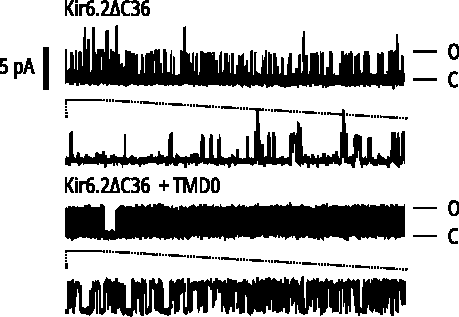
\includegraphics[width=\textwidth]{single_traces_tmd0.pdf}
	\end{subfigure}
	\vfill
	\begin{subfigure}[t]{0.45\textwidth}
		\caption{}\label{ch1fig:intrinsic_diagram}
		\centering
		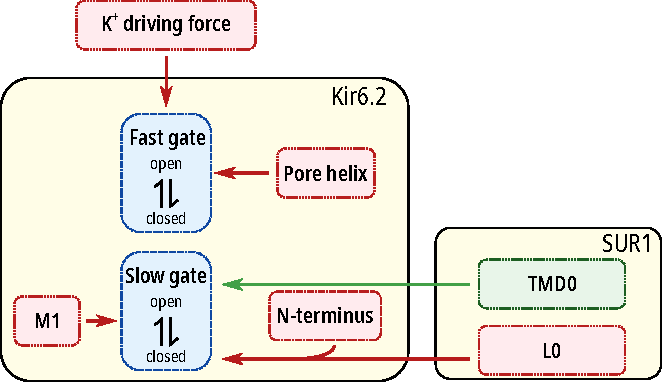
\includegraphics[width=\textwidth]{regulation_diagram_2.pdf}
	\end{subfigure}
	\hfill
	\begin{subfigure}[t]{0.45\textwidth}
		\caption{}\label{ch1fig:sur_shift}
		\centering
		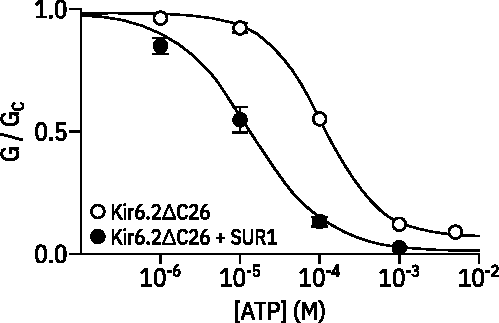
\includegraphics[width=\textwidth]{tucker_sur_shift.pdf}
	\end{subfigure}
	\caption[SUR1 modulates Kir6.2 gating]{
		\subref{ch1fig:singles_sur} Single channel recordings of excised patches from cultured cells either expressing Kir6.2 alone with the C-terminal 36 amino acids truncated (Kir6.2\textgreek{D}C36) or coexpressing wild-type Kir6.2 with SUR1.
		Adapted from (Enkvetchakul/Nichols, 2000).
		\subref{ch1fig:singles_tmd0} Single channel recordings of excised patches from cultured cells either expressing Kir6.2\textgreek{D}C36 alone or coexpressing Kir6.2\textgreek{D}C36 with the TMD0 region of SUR1.
		Adapted from (Pratt/Shyng, 2011).
		In both panels, currents were recorded in symmetrical 140 mM K\textsuperscript{+} at a membrane potential of -50 mV and openings are displayed as upward deflections.
		Note that the timescales differ slightly between panels as traces are from two separate papers.
		\subref{ch1fig:intrinsic_diagram} The intrinsic open-closed equilibrium of the pancreatic K\ATP{} channel pore is regulated by the K\textsuperscript{+} driving force and by the presence of different SUR1 domains.
		\subref{ch1fig:sur_shift} Concentration-response relationship of ATP from macroscopic currents excised from \textit{Xenopus} oocytes injected with either Kir6.2\textgreek{D}C26 mRNA alone (open circles), or a mixture of Kir6.2\textgreek{D}C26 and SUR1 mRNAs (closed circles).
		Response is given as the fraction of the slope conductance (G) remaining during exposure to ATP.
		Adapted from (Tucker/Ashcroft, 1997).
	}
\end{figure}

\citeauthor{babenko_two_1999} constructed a series of SUR1/SUR2A chimeras and characterised the changes in single channel kinetics that resulted from swapping different domains between the two isoforms of SUR.
They found that Kir6.2+SUR2A channels exhibited a far higher single channel $P_O$ than Kir6.2+SUR1 channels (0.91 and 0.64 respectively).
This difference could be attributed to increased burst durations and decreased interburst periods, while fast gating is indistinguishable.
They found that a chimerical construct replacing the N-terminal 291 amino acids of SUR1 with those of SUR2A was sufficient to recapitulate the single channel kinetics of full-length SUR2A, suggesting that this region is critical for specifying the intrinsic gating of K\ATP{}.

Later work established that truncations of SUR1 to TMD0 or TMD0-L0 fragments allowed expression of "mini-K\ATP{}" channels at the cell membrane \cite{babenko_sur_2003, chan_n-terminal_2003, fang_n-terminal_2006}.
The first two studies showed that expression of Kir6.2 with TMD0 alone (residues 1-195 or 1-196 of SUR1) essentially recapitulates the intrinsic gating characteristics of Kir6.2 expressed with full-length SUR1, restoring the increased open time duration and burst duration as compared to expression of Kir6.2 alone \cite{babenko_sur_2003, chan_n-terminal_2003}.
\citeauthor{fang_n-terminal_2006} later found that in their hands, mini-K\ATP{} channels formed from Kir6.2\textgreek{D}C and SUR1-TMD0 were similar to full-length K\ATP{} but they consistently observed differences in the burst durations.
This discrepancy may be, at least in part, due to differences in the heterologous expression system (COSm6 cells in \cite{babenko_sur_2003}, \textit{Xenopus} oocytes in \cite{fang_n-terminal_2006}).
Otherwise, the remaining difference between K\ATP{} and mini-K\ATP{} channels could either be due to differences in structural interactions due to the truncation, or could implicate a role for the ABC core domain in regulating slow gating \cite{fang_n-terminal_2006}.

Increasing the length of the SUR1 fragment to include the first section of the L0 linker (residues 1-232 of SUR1) results in a nearly constitutively open channel, with dramatically increased open time duration and few observable interburst closures \cite{babenko_sur_2003}.
The resulting $P_O$ of 0.93 reflects a near saturation of the slow gating process; as without changes to the fast gating there can be limited further increases in $P_O$ due to the flickery closure.
Increasing the length of the L0 linker included in the SUR1 truncation fragment results in a progressive decrease in the open time duration, burst length and $P_O$, although it never regresses to the kinetics observed in Kir6.2 expressed alone \cite{babenko_sur_2003}.
These findings suggest that while the TMD0 and the initial segment of L0 help to stabilise the open state of K\ATP{} channels, sections of the L0 linker act to destabilise the open state in some fashion \cite{babenko_sur_2003, puljung_cryo-electron_2018-1}.

One hypothesis for this destabilisation is that parts of the L0 linker interact with the N-terminus of Kir6.2 to regulate intrinsic gating of K\ATP{} channels \cite{koster_atp_1999, babenko_n-terminus_1999, reimann_involvement_1999-1, babenko_sur-dependent_2002}.
When Kir6.2\textgreek{D}C is expressed alone, deletion of the first 14 amino acids of the N-terminus of Kir6.2 does not affect single channel kinetics \cite{reimann_involvement_1999-1}.
However, in the presence of SUR1, truncations of up to the first 44 amino acids of the N-terminus reduces the frequency of transitions to the long closed state, increasing the $P_O$ \cite{reimann_involvement_1999-1, koster_atp_1999, babenko_n-terminus_1999}.
This effect increases with progressive truncations from \textgreek{D}N4 to \textgreek{D}N30, but increasing the truncation past this point does not appear to have additional effects.

\citeauthor{cukras_role_2002} conducted an alanine scan of positively charged residues in the N-terminus of Kir6.2.
They identified two residues in the proximal 30 amino acids which reduced $P_O$ when substituted (R4A, K5A) and two residues which increased $P_O$ when substituted (R16A, R27A).

Application of a synthetic peptide which contains the first 33 amino acids of the N-terminus of Kir6.2 to full-length K\ATP{} channels decreases the frequency of transitions to the closed state, in a manner comparable to truncation of the N-terminus \cite{babenko_sur-dependent_2002}.
This effect was dependent on the presence of SUR1, as with the N-terminal truncation experiments.
This finding suggests that the synthetic peptide competes with the endogenous N-terminal of Kir6.2 for an interaction within the K\ATP{} channel complex.

Finally, \citeauthor{craig_-frame_2009} investigated an in-frame deletion of five amino acids (28\textgreek{D}32) identified in neonatal diabetes patients.
This deletion resulted in K\ATP{} channels with increased $P_O$ only in the presence of SUR1; single Kir6.2\textgreek{D}C and Kir6.228\textgreek{D}32,\textgreek{D}C channel currents were indistinguishable.
The authors then made use of the 1-195 and 1-288 truncated SUR1 constructs described in reference \cite{babenko_sur_2003}, and determined that only when the L0 linker was present (i.e. SUR1 residues 1-288) was there a difference in intrinisc gating upon the 28\textgreek{D}32 deletion.

Together, these results provide evidence for interactions between SUR1 and the N-terminal of Kir6.2 which facilitate transitions to the long closed state of the channel \cite{babenko_sur_2003}.

Of course, when measuring currents from hundreds or thousands of K\ATP{} channels, it is not possible to distinguish between perturbations which alter fast gating and perturbations which alter slow gating; the current measured reflects the sum of both of these processes.
At a macroscopic level, anything which increases single channel open time or burst duration, or decreases the intraburst closed time or frequency of entering the interburst state will be indistinguishable.

\section{Ligand dependent regulation of the pancreatic K\ATP{} channel}

K\ATP{} channels are regulated by two classes of endogenous ligands (nucleotides and phosphoinositides) and a range of exogenous ligands (predominantly sulphonylureas and glinides) (Figure \ref{ch1fig:regulation_diagram}).
Thus far, the action of each of these ligands appears to exclusively affect the slow gating of channel \cite{proks_modeling_2009}.
While the binding of adenine nucleotides to the Kir6.2 binding site leads to closure of the pore, binding of nucleotides to the NBSs of SUR1 in the presence of Mg\textsuperscript{2+} activates the channel \cite{nichols_adenosine_1996-1, vedovato_nucleotide-binding_2015}.
The interplay between the action of nucleotides at these distinct sites (Figure \ref{ch1fig:sur_ctd}) determines the response of the K\ATP{} channel to metabolic changes, and therefore even subtle mutations or modifications to these sites can lead to diseases of insulin secretion.
Phosphoinositides present in cell membranes are also regulators of K\ATP{} function, a property which is shared amongst the Kir family of channels \cite{fan_anionic_1997, nichols_k_2006, hibino_inwardly_2010}.
PIP\textsubscript{2} especially stimulates the opening of K\ATP{}, and excision of membrane patches results in a decline of channel activity due to the loss of PIP\textsubscript{2} in the excised membrane over time \cite{proks_running_2016-2}.
Finally, in addition to allowing activation of the channel by Mg-nucleotides, proper assembly of Kir6.2 and SUR1 allows for highly sensitive inhibition of currents by sulphonylureas and glinides \cite{gribble_interaction_1997, ashcroft_new_2010}.

Proteins are inherently dynamic and sample a vast ensemble of accessible conformations \cite{boehr_role_2009}.
Techniques with high temporal resolution such as NMR spectroscopy have revealed the breadth of the energy landscape of macromolecules, and highlighted the ability of molecules at equilibrium to adopt a variety of conformational states \cite{mittermaier_new_2006}.
The K\ATP{} channel is no exception.
The ability of the channel to open and close in the absence of ligand (i.e. after channel rundown due to loss of PIP\textsubscript{2}) shows that at equilbrium, the K\ATP{} channel is able to exchange between open and closed states, albeit with a much higher occupancy of closed states \cite{ribalet_regulation_2000, proks_running_2016-2}.
One mechanism by which ligands are proposed to regulate the equilibrium of K\ATP{} channels (and macromolecules in general) is by being selective for particular conformations.
For example, PIP\textsubscript{2} will exhibit a higher binding affinity for an open state of the channel that it will for a closed state; and thus the presence of PIP\textsubscript{2} will selectively stabilise the open state of K\ATP{} channels.
This mechanism is the cornerstone of the MWC model of allostery \cite{monod_nature_1965-1, rubin_nature_1966, garcia_chapter_2011, marzen_statistical_2013}, and its assumptions and implications will be discussed in more detail in \ref{ch4}.
In this framework, the link between ligand binding and channel gating, sometimes called transduction, is the factor by which a ligand preferentially stabilises a particular conformation.
Figure \ref{ch1fig:regulation_diagram} is a simplified diagram of how ligands interact to regulate the K\ATP{} channel.
Briefly, $L$ describes the unliganded equilibrium between open and closed, while ligands which bind with affinity constants $K_X$ preferentially stabilise the open state by a factor $D_X > 1$ or the closed state by a factor $D_X < 1$.

\begin{figure}[h]
	\centering
	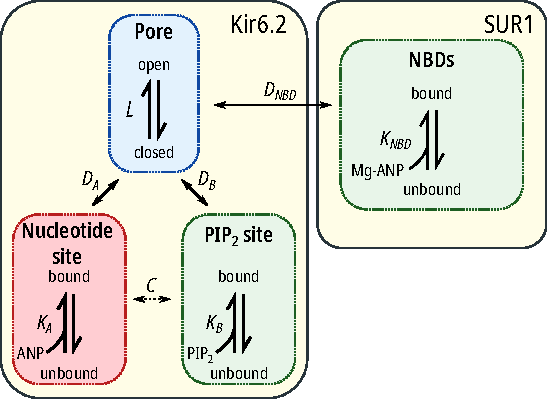
\includegraphics[width=0.7\textwidth]{regulation_diagram.pdf}
	\caption[Modes of regulation of K\ATP{}]{
	Adapted from \cite{puljung_cryo-electron_2018}.
	The open-closed equilibrium of the K\ATP{} channel pore (denoted as $L$) is energetically coupled to three different ligand binding sites.
	The four inhibitory nucleotide binding sites of Kir6.2 (labelled as NBS) bind either ATP or ADP (generalised to ANP) with an equilbrium binding constant $K_A$.
	The four stimulatory PIP\textsubscript{2} binding sites of Kir6.2 bind PIP\textsubscript{2} with an equilbrium binding constant $K_B$.
	The four stimulatory Mg-nucleotide binding site formed by the dimerisation of the NBDs of SUR1 (labelled as NBDs) bind either Mg-ATP or Mg-ADP (generalised to Mg-ANP) with an equilbrium binding constant $K_C$.
	Each binding domain interacts with the channel pore according to the factors $D_A$, $D_B$, and $D_{NBD}$ respectively.
	In addition, there is a potential coupling between the inhibitory nucleotide binding site of Kir6.2 and the stimulatory PIP\textsubscript{2} binding site of Kir6.2 described by the factor $C$.
	}\label{ch1fig:regulation_diagram}
\end{figure}

\subsection{Nucleotide regulation of the pancreatic K\ATP{} channel}

The physiological regulation of channel activity by nucleotides is the summed contribution of activation by Mg-nucleotides binding to the NBSs of SUR1, and inhibition by nucleotides binding to Kir6.2 \cite{nichols_adenosine_1996}.
To study these contributions experimentally, most research to date has relied on electrophysiological recordings of K\ATP{} currents.
Separating the contributions of the different classes of site has been achieved through a variety of methods.
Firstly, activation of the channel by Mg-nucleotides can be eliminated by removing Mg\textsuperscript{2+} ions from the solutions used to perfuse excised patches by inclusion of high concentrations of chelators such as EGTA \cite{gribble_mgatp_1998-1, proks_activation_2010-1}.
This experimental paradigm allows for the measurement of inhibition by nucleotides alone.
Secondly, activation of the channel by Mg-nucleotides can be isolated by introducing mutations which abolish nucleotide binding to Kir6.2 \cite{gribble_mgatp_1998-1, proks_activation_2010-1}.

Mutation of residues which are involved in nucleotide inhibition of the K\ATP{} channel can result in one of two functional effects.
In the first category are residues which, when substituted, reduce the sensitivity of the channel to nucleotide inhibition (i.e. increase the IC\textsubscript{50} for nucleotide inhibition) while not perturbing the intrinsic gating of the channel.
Mapping these residues to the the cryo-EM structures of ATP-bound K\ATP{} reveals that the residues in this category are invariably located close to the nucleotide binding site of Kir6.2.
The binding site is composed of part of the N-terminal region of one Kir6.2 subunit, and part of the C-terminal region of its neighbouring subunit.
Well characterised mutations of residues in this region of the N-terminus (R50 \cite{proks_involvement_1999, cukras_role_2002, john_molecular_2003, ribalet_molecular_2003, trapp_identification_2003, shimomura_mutations_2006}, G53 \cite{koster_dend_2008}) and C-terminus (I182 \cite{drain_katp_1998, koster_atp_2005, li_i182_2000}, K185 \cite{john_molecular_2003, ribalet_molecular_2003, trapp_identification_2003}, F333 \cite{tammaro_kir62_2005}, G334 \cite{drain_katp_1998, tammaro_kir62_2005, masia_atp-binding_2007-1, proks_activation_2010-1}) have no effects on single channel kinetics in the absence of nucleotide.
However, they are far less sensitive to inhibition by nucleotides.
The simplest hypothesis to explain this data given the location of the residues in the structures is that mutations of these residues perturb interactions between K\ATP{} and nucleotides, reducing the direct binding affinity of nucleotides for the inhibitory binding site (i.e. a reduction of $K_A$ in Figure \ref{ch1fig:regulation_diagram}).

Alternatively, mutations which do not affect intrinsic gating but reduce sensitivity to nucleotide inhibition may be affecting the relative selectivity of nucleotides for the closed state of the channel (i.e. $D_A$ approaches unity in Figure \ref{ch1fig:regulation_diagram}).
R201 was hypothesised to form part of the binding site as a cysteine \cite{proks_molecular_2004, antcliff_functional_2005} or histidine \cite{tammaro_functional_2006} substitution at this site results in reduced inhibition of K\ATP{} channels by nucleotides, without any changes in intrinsic gating .
Curiously, an alanine at this position results in K\ATP{} channels which exhibit both reduced sensitivity to ATP inhibition and reduced activation by PIP\textsubscript{2} \cite{shyng_structural_2000}.
Examining the cryo-EM structures suggests that this residue does not form direct contacts with bound ATP, and would therefore have to alter the nucleotide binding site allosterically - potentially by stabilising the short helix containing the critical F333 and G334 residues \cite{puljung_cryo-electron_2018}.
\citeauthor{ribalet_molecular_2003, john_molecular_2003} proposed that mutating R201 to an alanine instead acts by perturbing the preference of nucleotides for the closed state of the channel, increasing $D_A$.

The second category of residues are those which, when mutated, increase the $P_O$ of the channel and also affect the sensitivity of the channel to nucleotide inhibition.
This category is far larger, and these residues are found across both Kir6.2 and SUR1 structures.
Within the MWC framework in Figure \ref{ch1fig:regulation_diagram}, mutations which increase $L$ (and therefore increase the observed $P_O$) reduce the ability of nucleotides to inhibit the channel.
By increasing the stability of the open state, the selectivity of nucleotides for the closed state ($D_A < 1$) results in a decreased probability of nucleotide binding, and thus reducing inhibition.
Mutations within this category are difficult to fully characterise in the cell membrane environment due to the presence of phosphoinositides.
An observed increase in $P_O$ in an excised patch may either stem from an increase in $L$, or from an increase in $K_B$ or $D_B$.

Activation of K\ATP{} channels by Mg-nucleotides is not quite as trivial to measure in isolation.
The most common experimental paradigm used to isolate activatory effects is introducing a mutation into Kir6.2 which renders it insensitive to inhibition by nucleotides \cite{gribble_mgatp_1998-1, proks_activation_2010-1}.
Apllication of Mg-nucleotides to mutant channels such as Kir6.2-G334D then results in an increase in the burst duration and therefore the $P_O$ of K\ATP{} channels \cite{proks_activation_2010-1}.
This stimulatory effect is conferred by the NBSs of SUR1, as mutation of the Walker A motif in either NBS1 or NBS2 results in K\ATP{} channels which are no longer activated by Mg-nucleotides \cite{gribble_essential_1997,nichols_adenosine_1996}.

In ABC transporters, the conformational changes which allow substrate movement across the membrane are driven by ATP hydrolysis \cite{rees_abc_2009}.
In addition, there is strict coupling between ATP hydrolysis and channel gating in CFTR, an ABC family member which is in itself a chloride channel \cite{csanady_strict_2010-1}.
The NBDs of SUR1 are capable of hydrolysing ATP at rates comparable to that of CFTR \cite{matsuo_atp_1999, wet_studies_2007, puljung_cryo-electron_2018}.
\citeauthor{zingman_signaling_2001-1} used beryllium-fluoride and orthovanadate to stabilise the pre- and post-hydrolytic states of SUR1 respectively, and suggested that the post-hydrolytic state favoured channel opening.

However, \citeauthor{choi_testing_2008} analysed the microscopic reversibility of single-channel kinetics to determine whether ATP hydrolysis is coupled to channel gating.
Microscopic reversibility is a property of equilibrium systems such that their dynamics are time-reversible.
As ATP hydrolysis is irreversible and thus not in equilibrium, if channel gating is dependent on ATP hydrolysis it will not obey microscopic reversibility \cite{rothberg_testing_2001}.
Unlike for CFTR \cite{csanady_strict_2010-1}, \citeauthor{choi_testing_2008} found no evidence for ATP-dependent violations of microscopic reversibility in K\ATP{} channel gating, supporting the conclusion that ATP hydrolysis by the NBDs of SUR1 is not directly coupled to conformational changes of the channel.
In addition, Mg-ADP is sufficient to activate channel currents, obviating the need for ATP hydrolysis \cite{proks_activation_2010-1}.
It is most likely that the activatory function of Mg-nucleotides occurs in a similar manner as in inhibitory function of nucleotides; via an allosteric equilibrium effect on the channel pore ($D_{NBD}$ in Figure \ref{ch1fig:regulation_diagram}).

\subsection{PIP\textsubscript{2} regulation of the pancreatic K\ATP{} channel}

A conserved feature of Kir channels is that they are regulated by phosphoinositides, in particular PIP\textsubscript{2}, and Kir6.2 is no exception \cite{hibino_inwardly_2010, fan_anionic_1997, shyng_membrane_1998, baukrowitz_pip2_1998}.
Studying the nature of the regulation of K\ATP{} by PIP\textsubscript{2} is difficult experimentally due to the lack of control over PIP\textsubscript{2} concentrations, and our inability to precisely measure them.
Firstly, while the contaminating effects of intracellular nucleotides are removed by excision of a patch, the same is not true for PIP\textsubscript{2}.
The rundown of channel currents is largely attributable to dissociation and/or degradation of PIP\textsubscript{2} from the membrane patch, but rundown is a complex phenomenon and the relative amounts of PIP\textsubscript{2} in the membrane varies between patches and experimental conditions \cite{proks_running_2016-2}.
The hydrophobicity of PIP\textsubscript{2} means that perfusing a membrane patch results in accumulation of lipid in the membrane; it is impossible to reach an equilibrium with a known concentration.
An alternative is using analogs of PIP\textsubscript{2} with increased solubility due to shortening of the acyl chain length, such as dioctanoyl (diC\textsubscript{8}) PIP\textsubscript{2} \cite{rohacs_specificity_2003}.
While more soluble analogs are easier to work with and an experimenter can reach a quasi-equilibrium, we do not know how the concentration of diC\textsubscript{8} PIP\textsubscript{2} applied to a membrane equates to the concentration achieved in the membrane.
Another alternative is using polyamines such as neomycin as negative charge chelators; screening the negatively-charged phospholipid head groups present in the membrane away from their normal binding sites \cite{fan_anionic_1997, schulze_phosphatidylinositol_2003}.
This approach runs into the problems of both methods previously outlined; we do not know the precise correlation between the concentration of neomycin applied and the concentration of active, un-chelated PIP\textsubscript{2} in the membrane; and due to rundown it is impossible to reach a true equilibrium.

Despite all these complexities, there is still a great deal of research exploring how PIP\textsubscript{2} regulates K\ATP{} channel gating.
PIP\textsubscript{2} stimulates K\ATP{} channel currents by increasing channel open time and burst duration, and reduces the sensitivity of K\ATP{} channel currents to inhibition by nucleotides \cite{fan_phosphoinositides_1999, baukrowitz_pip2_1998, shyng_membrane_1998, fan_phosphoinositides_1999, enkvetchakul_kinetic_2000}.
The stimulatory effect occurs in the absence of SUR1, as the $P_O$ of Kir6.2\textgreek{D}C or Kir6.2-cGFP expressed alone is still enhanced by perfusion of PIP\textsubscript{2} \cite{fan_phosphoinositides_1999, enkvetchakul_kinetic_2000}.
However, the presence of SUR1 appears to enhance the ability of PIP\textsubscript{2} to stimulate channel currents \cite{baukrowitz_pip2_1998, shyng_membrane_1998, fan_phosphoinositides_1999, enkvetchakul_kinetic_2000}.
This enhancement has been proposed to occur through the interaction between the N-terminal of Kir6.2 and TMD0 of SUR1, and may account (at least in part) for the increase in 'intrinisc' $P_O$ observed when Kir6.2 and SUR1 are coexpressed \cite{pratt_n-terminal_2011}.
\citeauthor{pratt_n-terminal_2011} introduced a mutation (E128K) into the TMD0 region of SUR1 and found that K\ATP{} channels formed either with full-length mutant SUR1 or mutant TMD0 exhibited drastically reduced $P_O$ when compared to their wild-type counterparts.
In addition, the E128K mutation reduced the activation of channel currents by PIP\textsubscript{2}, and exposure to PIP\textsubscript{2} did not reduce the sensitivity of E128K channels to nucleotide inhibition.
These findings highlight the complexity of the regulatory role of SUR1, and also the difficulty in separating effects on intrinsic channel gating from effects on PIP\textsubscript{2} regulation, given the difficulty in measuring and controlling the latter.

The second functional aspect of PIP\textsubscript{2} modulation is its effects on sensitivity of K\ATP{} channels to nucleotide inhibition.
Application of PIP\textsubscript{2} reduces the ability of nucleotides to inhibit K\ATP{} channels, and reduction of PIP\textsubscript{2} activity from rundown or application of neomycin increases the ability of nucleotides to inhibit K\ATP{} channels \cite{baukrowitz_pip2_1998, shyng_membrane_1998, fan_phosphoinositides_1999, enkvetchakul_kinetic_2000}.
In addition, photoaffinity labelling of Kir6.2 by ATP analogs is reduced in the presence of phosphoinositides \cite{wang_compromised_2002}.
This phenomenon can be explained by the allosteric effects of increasing channel $P_O$, which would result in a corresponding decrease in nucleotide binding and inhibition due to the energetic coupling of the nucleotide binding site and the channel pore ($D_A$ in Figure \ref{ch1fig:regulation_diagram}) \cite{proks_modeling_2009}.
However, it has also been hypothesised that there is an additional interaction between nucleotides and PIP\textsubscript{2} which is not mediated through energetic coupling to the channel pore ($C$ in Figure \ref{ch1fig:regulation_diagram}) \cite{fan_phosphoinositides_1999, proks_modeling_2009, haider_identification_2007}.
This interaction could be due to direct competition between PIP\textsubscript{2} and nucleotides for the same site, or by local allosteric interactions which energetically disfavour binding of one ligand when the other is already bound.

While the cryo-EM structures of K\ATP{} were not able to capture a PIP\textsubscript{2}-bound state, there is a crystal structure of Kir2.2 complexed with PIP\textsubscript{2} which suggests that the Kir6.2 PIP\textsubscript{2} binding site is not the same as the nucleotide binding site \cite{hansen_structural_2011}.
This is supported by mutagenic electrophysiological studies, which show that substitutions at residues which alter nucleotide sensitivity but not $P_O$ also do not affect activation of channel currents by PIP\textsubscript{2} (with the notable exception of R201, which is discussed previously) \cite{fan_anionic_1997, shyng_structural_2000, schulze_phosphatidylinositol_2003, haider_identification_2007}.
This does not rule out the possibility of separate but overlapping sites for nucleotide and PIP\textsubscript{2} binding, and whether nucleotides and PIP\textsubscript{2} are able to simultaneously bind to the same subunit remains an open question \cite{enkvetchakul_gating_2003-2, proks_modeling_2009}.

\section{Fluorescence methods in ion channel research}

\subsection{Fluorescence as a tool}

\subsection{Forster resonance energy transfer}

\subsection{Unnatural amino acid incorporation}

\chapter{\label{ch:2-methods}Methods}

\graphicspath{{figures/ch2/}}

\minitoc 

\section{Molecular biology.}
Human Kir6.2 and SUR1 were subcloned into pcDNA4/TO and pCGFP\_EU vectors for expression of wild-type and GFP-tagged constructs, respectively.
pcDNA4/TO and pANAP were obtained from Addgene.
peRF1-E55D and pCGFP\_EU were kind gifts from the Chin Laboratory (MRC Laboratory of Molecular Biology, Cambridge, UK) and the Gouaux Laboratory (Vollum Institute, Oregon, USA) respectively.
Amber stop codons and point mutations were introduced using the QuikChange XL system (Stratagene; San Diego, CA).
All constructs were confirmed by DNA sequencing (DNA Sequencing and Services, University of Dundee, Scotland).

\section{Cell culture and channel expression}
HEK-293T cells were obtained from and verified/tested for mycoplasma by LGC standards (ATTC CRL-3216, Middlesex, UK).
Our working stock tested negative for mycoplasma contamination using the MycoAlert Mycoplasma Detection Kit (Lonza Bioscience; Burton on Trent, UK).
Cells were plated onto either poly-L-lysine coated borosilicate glass coverslips (VWR International; Radnor, PA) or poly-D-lysine coated glass-bottomed FluoroDishes (FD35-PDL-100, World Precision Instruments).
ANAP-tagged Kir6.2 constructs were labelled using amber stop codon suppression as described by Chatterjee et al.
Transfections were carried out 24 hours after plating using TransIT-LT1 (Mirus Bio LLC; Madison, WI) at a ratio of 3 \si{\micro\litre} per \si{\micro\gram} of DNA.
Unless specified otherwise, all transfections included a Kir6.2 construct with an amber stop codon (TAG) at position 311 (Kir6.2-W311\textsuperscript{TAG}), SUR1, pANAP and eRF1-E55D in the ratio 0.5:1.5:1:1.
Transfected cells cultured in Dulbecco’s Modified Eagle Medium (Sigma; St. Louis, MO) + 10\% foetal bovine serum, \SI{100}{\Unit\per\milli\litre} penicillin and \SI{100}{\micro\gram\per\milli\litre} streptomycin (Thermo Fisher Scientific; Waltham, MA) supplemented with \SI{20}{\milli\Molar} ANAP (free acid, AsisChem; Waltham, MA).
Cells were incubated at \SI{33}{\degreeCelsius} and in the presence of \SI{300}{\micro\Molar} tolbutamide to enhance protein expression and channel trafficking to the plasma membrane.
eRF1-E55D was included to increase efficiency of ANAP incorporation.
Experiments were carried out 2-4 days after transfection.
We also expressed constructs labelled with ANAP at positions I182, F183, F198, and I210.
Kir6.2-F183*, Kir6.2-F198*, and Kir6.2-I210* co-expressed with SUR1 did not produce sufficient currents for subsequent experimentation.
Mutations at I182 are known to produce profound effects on nucleotide inhibition of K\textsubscript{ATP}.
Thus, we did not consider this site for further experimentation.

\section{Western blots}
Transfected HEK-293T cells grown in 6-well plates were harvested in cold PBS (Life Technologies Limited; Paisley, UK), pelleted at 0.2 x g for 2.5 minutes and resuspended in lysis buffer containing 0.5\% Triton X-100, \SI{100}{\milli\Molar} potassium acetate, and a cOmplete protease inhibitor tablet (1 tablet/\SI{50}{\milli\litre}, Roche; Basel, Switzerland), buffered to pH 7.4.
After a 30-minute benzonase (Sigma) treatment at room temperature, samples were mixed with a DTT containing reducing agent and loading buffer (NuPAGE, Invitrogen; Carlsbad, CA) and run on a precast Bis-Tris 4-12\% poly-acrylamide gel at \SI{200}{\volt} for 40 minutes.
Proteins were wet transferred overnight onto polyvinylidene difluoride (PVDF) membranes (Immobilon P, Merck Millipore; Burlington, VT) in \SI{25}{\milli\Molar} Tris, \SI{192}{\milli\Molar} glycine, 20\% methanol, and 0.1\% SDS at \SI{10}{\volt} on ice.
Membranes were blocked with 5\% milk in TBS-Tw (\SI{150}{\milli\Molar} NaCl, 0.05\% Tween 20, \SI{25}{\milli\Molar} Tris, pH 7.2) before staining for 30 minutes with a 1:1000 dilution of rat anti-HA monoclonal antibody in TBS-Tw (clone 3F10, Roche).
After washing with TBS-Tw, membranes were incubated for 30 minutes with a 1:20,000 dilution of HRP-conjugated goat anti-rat polyclonal antibodies in TBS-Tw (Jackson ImmunoResearch; Ely, UK).
Detection was performed using the SuperSignal West Pico Chemiluminescent Substrate (Thermo Fisher) and a C-DiGit Blot Scanner (Licor Biosciences; Lincoln, NE).
Analysis was performed using custom code written in Python.

To confirm our ability to express full-length Kir6.2*-GFP, we performed western blots for HA-tagged Kir6.2 constructs in detergent-solubilized HEK-293T cells (Figure 1—Figure supplement 1C).
The HA tag plus a short linker (YAYMEKGITDLAYPYDVPDY) was inserted in the extracellular region following helix M1 of Kir6.2 between L100 and A101.
Transfection of wild-type Kir6.2-HA or Kir6.2-HA-GFP resulted in two bands on the western blots.
The upper bands were close to the expected sizes for full-length Kir6.2-HA and Kir6.2-HA-GFP (\SI{46}{\kilo\dalton} and \SI{77}{\kilo\dalton}, respectively).

We consistently observed a lower molecular weight band as well.
This band must correspond to an N-terminally truncated Kir6.2 product, as the apparent molecular weight shifted with addition of the C-terminal GFP tag.
Based on the molecular weight, we predict that the truncated protein product initiated from a start codon in the first transmembrane domain.
Therefore, we believe it is unlikely that this protein would form functional channels or traffic to the plasma membrane.
When Kir6.2-W311\textsuperscript{TAG}-HA or Kir6.2-W311\textsuperscript{TAG}-HA-GFP were co-transfected with SUR1, pANAP, and eRF1-E55D, and cells were cultured in the presence of ANAP, the western blots were similar to wild-type Kir6.2-HA or Kir6.2-HA-GFP.
Over 90\% full-length Kir6.2*-HA-GFP was produced under these conditions (Figure 1—Figure supplement 1D).
We were unable to quantify the percentage of full-length Kir6.2*-HA produced as the C-terminally truncated band resulting from termination at the TAG codon was very similar in size to the N-terminally truncated band.
Co-expression with SUR1 increased the percentage of full-length Kir6.2*-HA-GFP produced (Figure 1—Figure supplement 1D).
In the absence of ANAP, we did not observe any full-length Kir6.2, indicating that there was no read-through of the amber (TAG) stop codon (Figure 1—Figure supplement 1D).

\section{Confocal microscopy}
Confocal imaging was performed using a spinning-disk system (Ultra-VIEW VoX, PerkinElmer; Waltham, MA) mounted on an IX81 microscope (Olympus; Southend-on-Sea, UK) with a Plan Apo 60x oil immersion objective (NA = 1.4), provided by the Micron Advanced Bioimaging Unit, Oxford.
Transfected HEK-293T cells were incubated for 15 minutes with \SI{1}{\nano\Molar} CellMask Deep Red (Thermo Fisher) to stain plasma membranes before washing with PBS and imaging.
ANAP was excited with a solid-state laser at \SI{405}{\nano\Molar}.
GFP and CellMask were excited with an argon laser at \SI{488}{\nano\Molar} and \SI{633}{\nano\Molar} respectively.
Images were captured on an EMCCD camera (ImagEM; Hamamatsu Photonics; Welwyn Garden City, UK) binned at 2 x 2 pixels and analysed using Python.
A median filter with a box size of 32 x 32 pixels was applied to improve the signal-to-noise ratio by reducing background fluorescence.

We examined the surface expression of our ANAP-labelled constructs using confocal microscopy (Figure 1—Figure supplement 1A,B).
When Kir6.2-W311\textsuperscript{TAG}-GFP was co-transfected with SUR1 along with pANAP and eRF1-E55D in the presence of ANAP, the ANAP and GFP fluorescence were co-localized at the plasma membrane.
When wild-type Kir6.2-GFP was transfected under the same conditions, only GFP fluorescence was observed at the plasma membrane.
ANAP fluorescence was diffuse and confined to the cytoplasm or intracellular structures.
Thus, the plasma-membrane ANAP signal was specific for Kir6.2*-GFP.

\section{Surface expression assays}
We measured surface expression of HA-tagged Kir6.2 subunits using an approach outlined by Zerangue et al.
Cells were plated on \SI{19}{\milli\metre} coverslips coated with poly-L-lysine and transfected as described above.
Following incubation, cells were rinsed with PBS before fixation with 10\% formalin for 30 minutes at room temperature.
After washing again, cells were blocked with 1\% BSA in PBS for 30 minutes at \SI{4}{\degreeCelsius} before a 1-hour incubation at \SI{4}{\degreeCelsius} with a 1:1000 dilution (in PBS) of rat anti-HA monoclonal antibodies.
Cells were then washed 5 times on ice with 1\% BSA in PBS followed by a 30-minute incubation at \SI{4}{\degreeCelsius} with a 1:2000 dilution of HRP-conjugated goat anti-rat polyclonal antibodies.
Cells were washed 5 times in PBS + 1\% BSA and 4 times in PBS.
Coverslips were removed from the culture dishes and placed in clean, untreated dishes for measurement.
\SI{300}{\micro\litre} of SuperSignal ELISA Femto Maximum Sensitivity Substrate (Thermo Fisher) was added to each sample and the luminescence was measured using a Glomax 20/20 Luminometer (Promega; Madison, WI) after a 10 second incubation.

HEK-293T cells were transfected with Kir6.2 constructs with or without a TAG stop codon corresponding to position 311.
Cells were co-transfected with pANAP and eRF1-E55D in the presence or absence of SUR1 and cultured with or without ANAP.
Wild-type Kir6.2-HA and Kir6.2-HA-GFP in the presence of SUR1 were included as positive controls.
Kir6.2 constructs with no HA tag served as negative controls.
In the presence of ANAP, we observed strong trafficking of Kir6.2*-HA-GFP to the plasma membrane, but much less trafficking of Kir6.2*-HA (Figure 1—Figure supplement 1E).
When cells were cultured in the absence of ANAP, we observed little to no Kir6.2 surface expression from cells that were transfected with Kir6.2-W311\textsuperscript{TAG}-HA or Kir6.2-W311\textsuperscript{TAG}-HA-GFP, suggesting that prematurely truncated constructs did not traffic to the plasma membrane.
In the absence of SUR1, surface expression was weak for both wild-type and tagged constructs, despite the reported ability of Kir6.2-GFP to traffic to the plasma membrane in the absence of SUR1.

\section{Epifluorescence imaging and spectroscopy}
Epifluorescence imaging and spectroscopy were performed using a Nikon Eclipse TE2000-U microscope with a 60x water immersion objective (Plan Apo VC, NA = 1.2, Nikon; Kingston upon Thames, UK) or a 100x oil immersion objective (Nikon, Apo TIRF, NA = 1.49).
Imaging of ANAP was performed using a \SI{385}{\nano\metre} LED source (ThorLabs; Newton, NJ) with a \SI{390/18}{\nano\metre} band-pass excitation filter, an MD416 dichroic and a \SI{479/40}{\nano\metre} band-pass emission filter (all from ThorLabs).
GFP was imaged using a \SI{490}{\nano\metre} LED source (ThorLabs) with a \SI{480/40}{\nano\metre} band-pass excitation filter, a DM505 dichroic, and a \SI{510}{\nano\metre} long-pass emission filter (all from Chroma; Bellows Falls, VT).
Fluorescence spectra were collected by exciting ANAP as above but using a \SI{400}{\nano\metre} long-pass emission filter (ThorLabs), then passing emitted light through an IsoPlane 160 Spectrometer (Princeton Instruments; Trenton, NJ) with a \SI{300}{\gram\per\milli\metre} grating.
Images were collected with \SI{1}{\second} exposures on a Pixis 400BR\_eXcelon CCD (Princeton Instruments).

\section{Electrophysiology.}
Patch pipettes were pulled from thick-walled borosilicate glass capillaries (GC150F-15, Harvard Apparatus; Holliston, MA) to a resistance of \SIrange{1.5}{2.5}{\mega\ohm} when filled with pipette solution.
Currents were recorded at \SI{-60}{\milli\volt} from excised inside-out patches using an Axopatch 200B amplifier equipped with a Digidata 1322A digitizer and using pClamp 10 software (Molecular Devices; San Jose, CA).
Currents were low-pass filtered at \SI{5}{\kilo\hertz} and digitized at \SI{20}{\kilo\hertz}.
The bath solution (intracellular) contained \SI{140}{\milli\Molar} KCl, \SI{10}{\milli\Molar} HEPES, \SI{1}{\milli\Molar} EDTA and \SI{1}{\milli\Molar} EGTA (pH 7.3 with KOH).
The pipette solution (extracellular) contained \SI{140}{\milli\Molar} KCl, \SI{10}{\milli\Molar} HEPES and \SI{1}{\milli\Molar} EDTA (pH 7.4 with KOH).
All experiments were carried out in Mg\textsuperscript{2+}-free conditions.
Currents were leak corrected using the current remaining in bath solution containing \SI{5}{\milli\Molar} barium acetate at \SI{+60}{\milli\volt}, assuming a linear leak with a reversal potential of \SI{0}{\milli\volt}.
Inhibition was calculated and corrected for rundown by alternating test concentrations of nucleotide solution with nucleotide-free solution, then expressing the test currents as a fraction of the average of the control currents before and after the test solution as described previously.

\section{FRET calculations}
We calculated the expected FRET efficiency between ANAP incorporated at amino acid position 311 and a docked TNP-ATP molecule as described previously.
The equivalency between FRET efficiency (measured as ANAP quenching) and nucleotide binding is based on two main assumptions.
Firstly, we assume that the observed quenching from a bound nucleotide does not differ dramatically between open and closed states of the channel.
As there is no open-state structure of K\textsubscript{ATP}, we do not know exactly how much relative movement would occur between a bound TNP-ATP and Kir6.2-W311.
However, based on cryo-EM structures of apo and nucleotide-bound Kir6.2 we do not expect to see a change in the distance between these two positions.

Secondly, we assume that the ANAP and TNP-ATP molecules on each subunit do not undergo energy transfer with those on other subunits to an extent which would dramatically change the observed quenching.
At saturating TNP-ATP concentrations, where each ANAP-labelled site on Kir6.2 is occupied, FRET between ANAP and the closest acceptor will be kinetically favoured and the overall FRET efficiency will not be affected by cross-talk between neighbouring sites.
In the limiting case, at low TNP-ATP concentrations, one would expect a large proportion of Kir6.2 tetramers (with four ANAP-labelled binding sites) bound to only a single TNP-ATP molecule.
In this case, we expect a 4\% overestimation of nucleotide binding as calculated using a numerical method to simulate a single TNP-ATP acceptor with multiple ANAP donors based on the distances calculated from our docking.
This may have resulted in our binding curves becoming artifically shallow at low concentrations.
However, this difference is not significant in the context of our measurements as it is smaller than the observed error of our measurements at low TNP-ATP concentrations.

\section{Unroofed binding measurements.}
Unroofed membranes were prepared as described previously.
A coverslip plated with transfected HEK-293T cells was removed from the culture media and rinsed with PBS.
The coverslip was then briefly sonicated using a probe sonicator (Vibra-cell; Newtown, CT) leaving behind adherent plasma membrane fragments.
Cells cultured on FluoroDishes were rinsed and sonicated directly in the dish.
Unroofed membrane fragments were nearly invisible in bright-field images and identified by their GFP and ANAP fluorescence.
Fluorescent TNP-nucleotides (Jena Bioscience; Jena, Germany) were diluted in bath solution and perfused onto unroofed membranes using a valve controlled microvolume superfusion system (\si{\micro}Flow, ALA Scientific Instruments; Farmingdale, NY).

Fluorescence spectra were collected as described above.
A region of interest corresponding to the membrane fragment was manually selected and line-averaged for each wavelength.
A similarly sized region of background was selected and averaged, then subtracted from the spectrum of interest.
After subtraction, ANAP intensity was calculated by averaging the fluorescence intensity measured between \SI{469.5}{\nano\metre} and \SI{474.5}{\nano\metre}.
Bleaching was corrected by fitting the normalised ANAP intensity of exposures taken during perfusion with nucleotide-free solution to a single exponential decay of the form
\begin{equation} \label{eq:bleaching}
    \frac{F}{F_{max}} = ae^{kt} + (1 - a)
\end{equation}
then using the fit to correct the intensity of exposures taken during perfusion with test nucleotide solutions.

Some experiments were excluded from further analysis due to obvious cross-contamination between different solutions within the \si{\micro}Flow superfusion system.
These were identified by noticeable colour changes in the solution in the delivery tubes.

\section{Patch-clamp fluorometry.}
The tip of the patch pipette was centred on the slit of the spectrometer immediately after patch excision.
Currents were measured as described above.
Fluorescence emission spectra from the excised patch were acquired concurrently with current measurements, both during test solution application as well as nucleotide-free solution.
Background subtraction was slightly imperfect due to the exclusion of TNP-ATP from volume of the glass of the pipette, resulting in spectra that have negative intensities at the TNP-ATP peak at high nucleotide concentrations.
However, this over-subtraction does not affect the size of the ANAP peak, which we used to quantify nucleotide binding.

ANAP bleaching was corrected as for the unroofed binding experiments with Equation \ref{eq:bleaching} (Figure 2-Figure supplement 3A).
Due to the lower signal-to-noise ratio for PCF compared to the unroofed membranes, we performed experiments from both high-to-low and low-to-high TNP-ATP concentrations to minimise artifacts from our bleaching corrections.
Kir6.2*-GFP + SUR1 showed consistent bleaching time courses (Figure 2-Figure supplement 3B) and an average of 34\% of the initial ANAP fluorescence intensity remained at the end of each experiment (Figure 2-Figure supplement 3C).

Some experiments were excluded from further analysis due to low fluorescence intensity, as we were concerned about a low signal to noise ratio influencing our results.

\section{Data processing and presentation.}
Raw spectrographic images and current traces were pre-processed in Python and Clampfit (Axon) before analysis with R.
Where applicable, all experimental data points are displayed in each figure.
The number of experiments is reported in the figure legends and tables.
To help visualise uncertainty and prevent some data points being hidden, they are arranged with a small amount of horizontal jitter; vertical position remains unaffected.
Unless otherwise stated, summary statistics are overlaid as the mean with error bars representing the standard error of the mean.
Where these error bars are not visible, they are smaller than the size of the point used for the mean.

Hill fits to fluorescence quenching were nonlinear least-squares fits to the following equation:
\begin{equation} \label{eq:hill}
    \frac{y}{y_{max}} = 1 - E_{max} + \frac{E_{max}}{1 + 10^{(EC_{50} - [TNPATP]) \cdot h}}
\end{equation}
where $y$ represents normalised fluorescence intensity and $EC_{50}$ and $[TNPATP]$ are $\log_{10}$ values.
Current inhibition data were fit to the same equation but with $y$ representing normalised current magnitude, $IC_{50}$ instead of $EC_{50}$, and $I_{max}$ instead of $E_{max}$.

\section{Computational docking.}
Computational docking of TNP-ATP into the nucleotide binding site of Kir6.2 was performed using AutoDock-Vina and Pymol (Schrödinger, LLC; New York, NY).
11 TNP-ATP structures from the Protein Data Bank (PDB accession \#s 1I5D, 3AR7, 5NCQ, 5SVQ, 5XW6, 2GVD, 5A3S, 2PMK, and 3B5J) were used as starting poses and a 15x11.25x15 \si{\angstrom} box was centred on the ATP bound to Kir6.2 in PDB accession \#6BAA.
Protonation states for each residue were assigned using PDB2PQR and PROPKA 3.0.
The modal highest-scoring pose from the docking run was selected (PDB accession \#5XW6) and distances were measured from a pseudo atom at the centre of the fluorescent moiety.
TNP-ATP (PDB \#3AR7) was positioned into the first nucleotide binding domain of SUR1 (PDB \#6PZI) using the alignment tool in Pymol.

\section{Chemicals and stock solutions.}
Unless otherwise noted, all chemicals were obtained from Sigma.
TNP-ATP was obtained as a \SI{10}{\milli\Molar} aqueous stock from Jena Bioscience and stored at \SI{-20}{\degreeCelsius}. \SI{1}{\milli\Molar} aqueous stocks of ANAP-TFA were prepared by dissolving the free acid in \SI{30}{\milli\Molar} NaOH, and were stored at \SI{-20}{\degreeCelsius}. Tolbutamide stocks (\SI{50}{\milli\Molar}) were prepared in \SI{100}{\milli\Molar} KOH and stored at \SI{-20}{\degreeCelsius}.



%% APPENDICES %% 
% Starts lettered appendices, adds a heading in table of contents, and adds a
%    page that just says "Appendices" to signal the end of your main text.
\startappendices
% Add or remove any appendices you'd like here:
\chapter{\label{ch:8-appendix}Appendices} 

\graphicspath{{figures/appendix/}}

\begin{figure}[h]
	\centering
	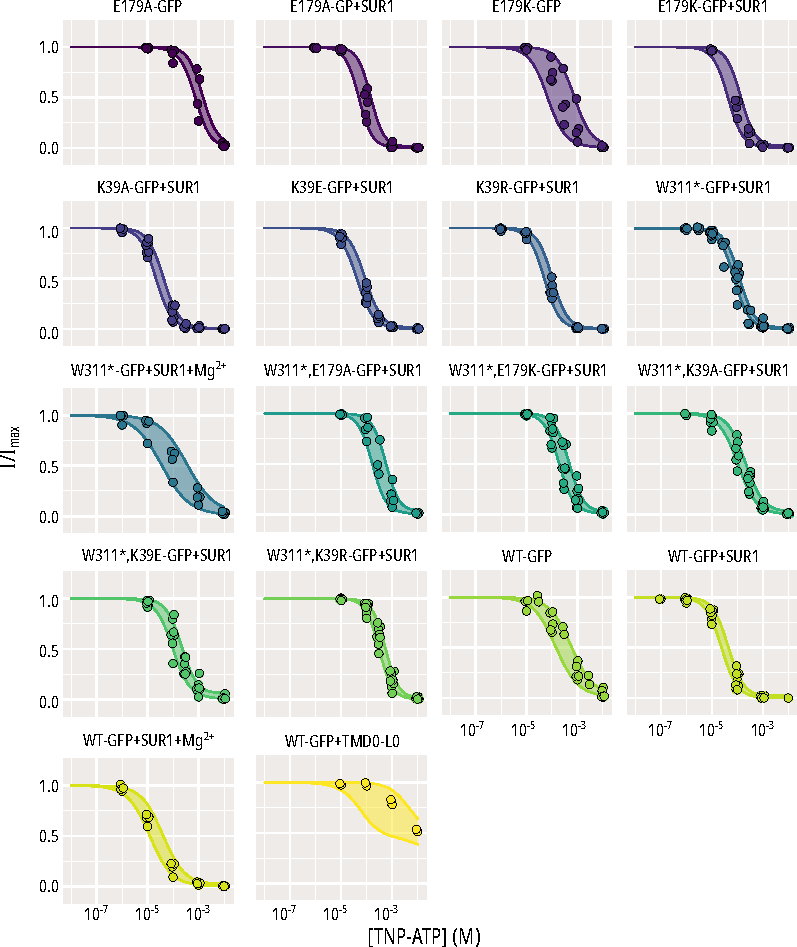
\includegraphics[width=\textwidth]{all_atp_fits.pdf}
	\caption[ATP inhibition population hill fits]{
	}
	\label{apxfig:atp_inhib_1}
\end{figure}

\begin{figure}[h]
	\centering
	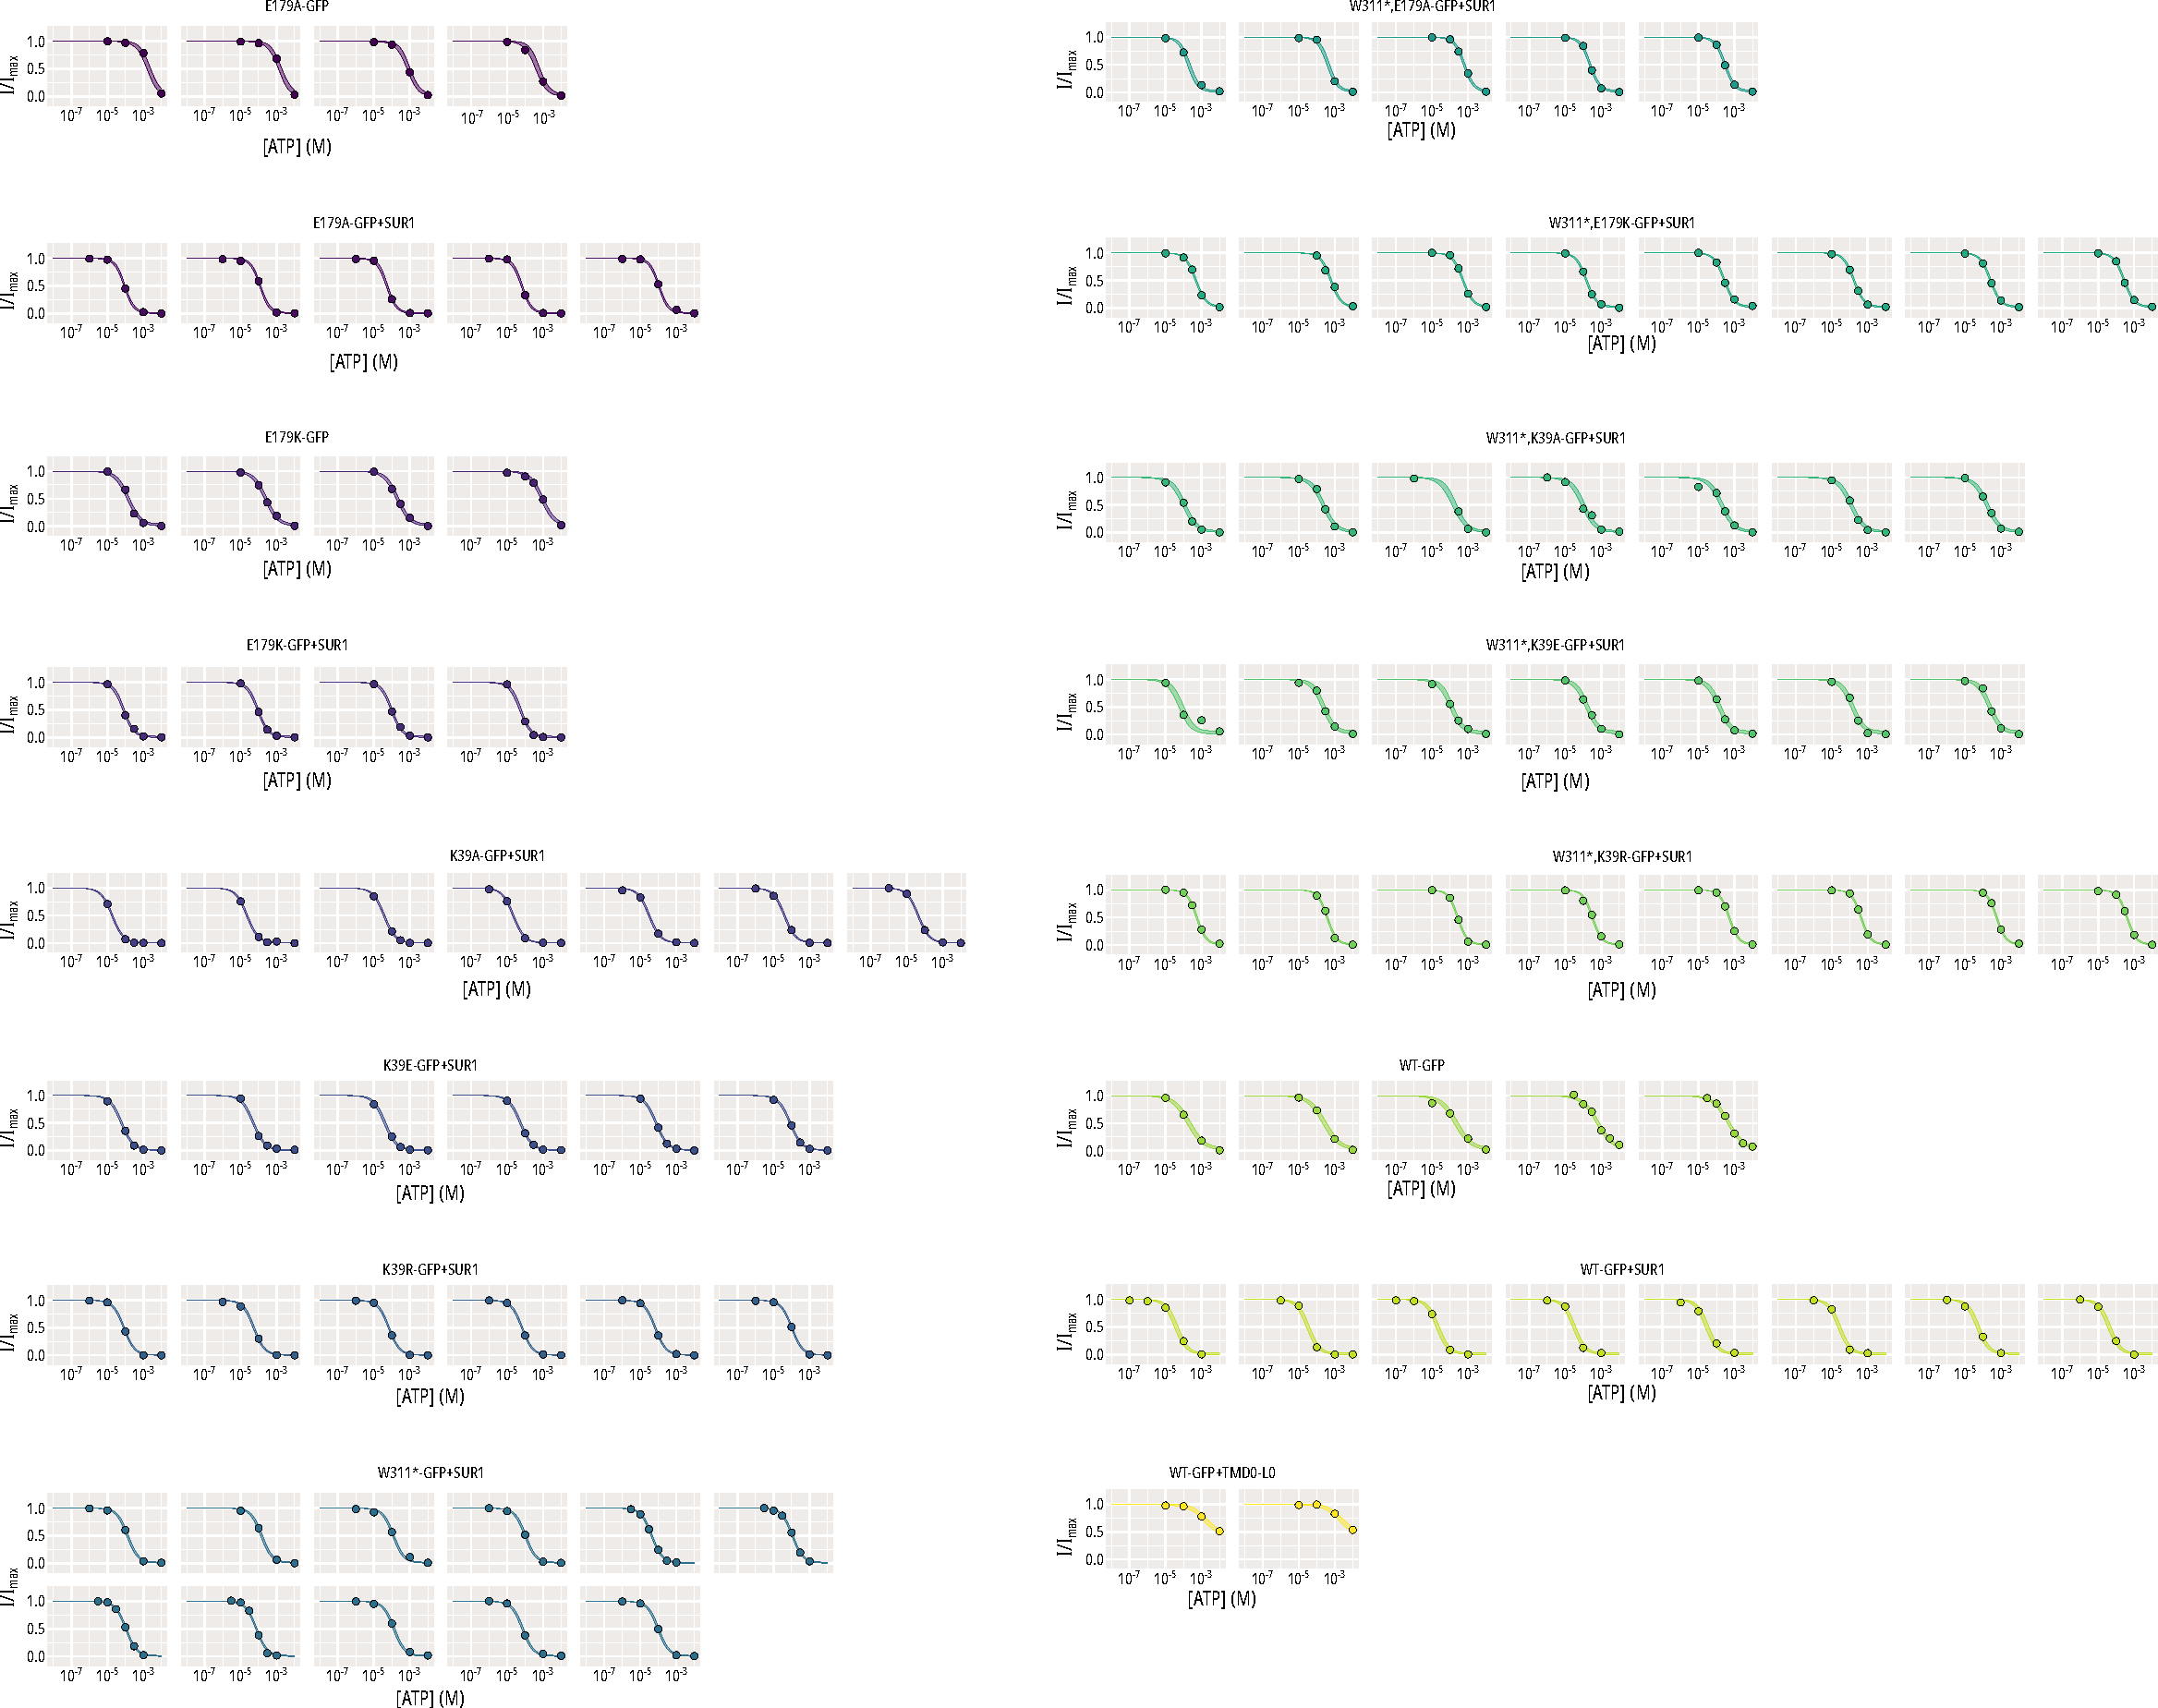
\includegraphics[width=\textwidth]{all_atp_fits_2.pdf}
	\caption[ATP inhibition sample hill fits]{
	}
	\label{apxfig:atp_inhib_2}
\end{figure}

\begin{figure}[h]
	\centering
	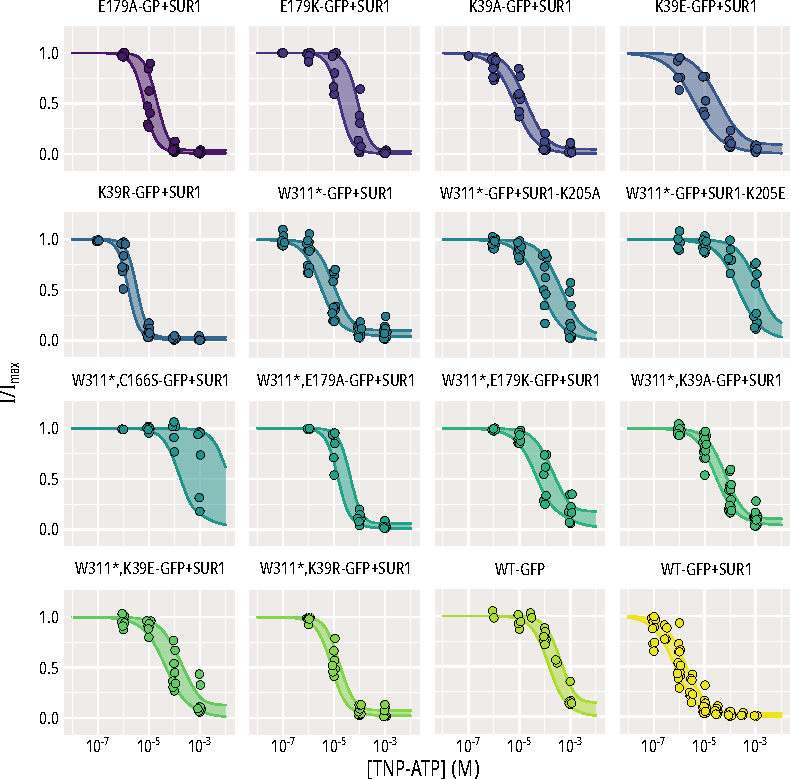
\includegraphics[width=\textwidth]{all_tnpatp_fits.pdf}
	\caption[TNP-ATP inhibition population hill fits]{
	}
	\label{apxfig:tnpatp_inhib_1}
\end{figure}

\begin{figure}[h]
	\centering
	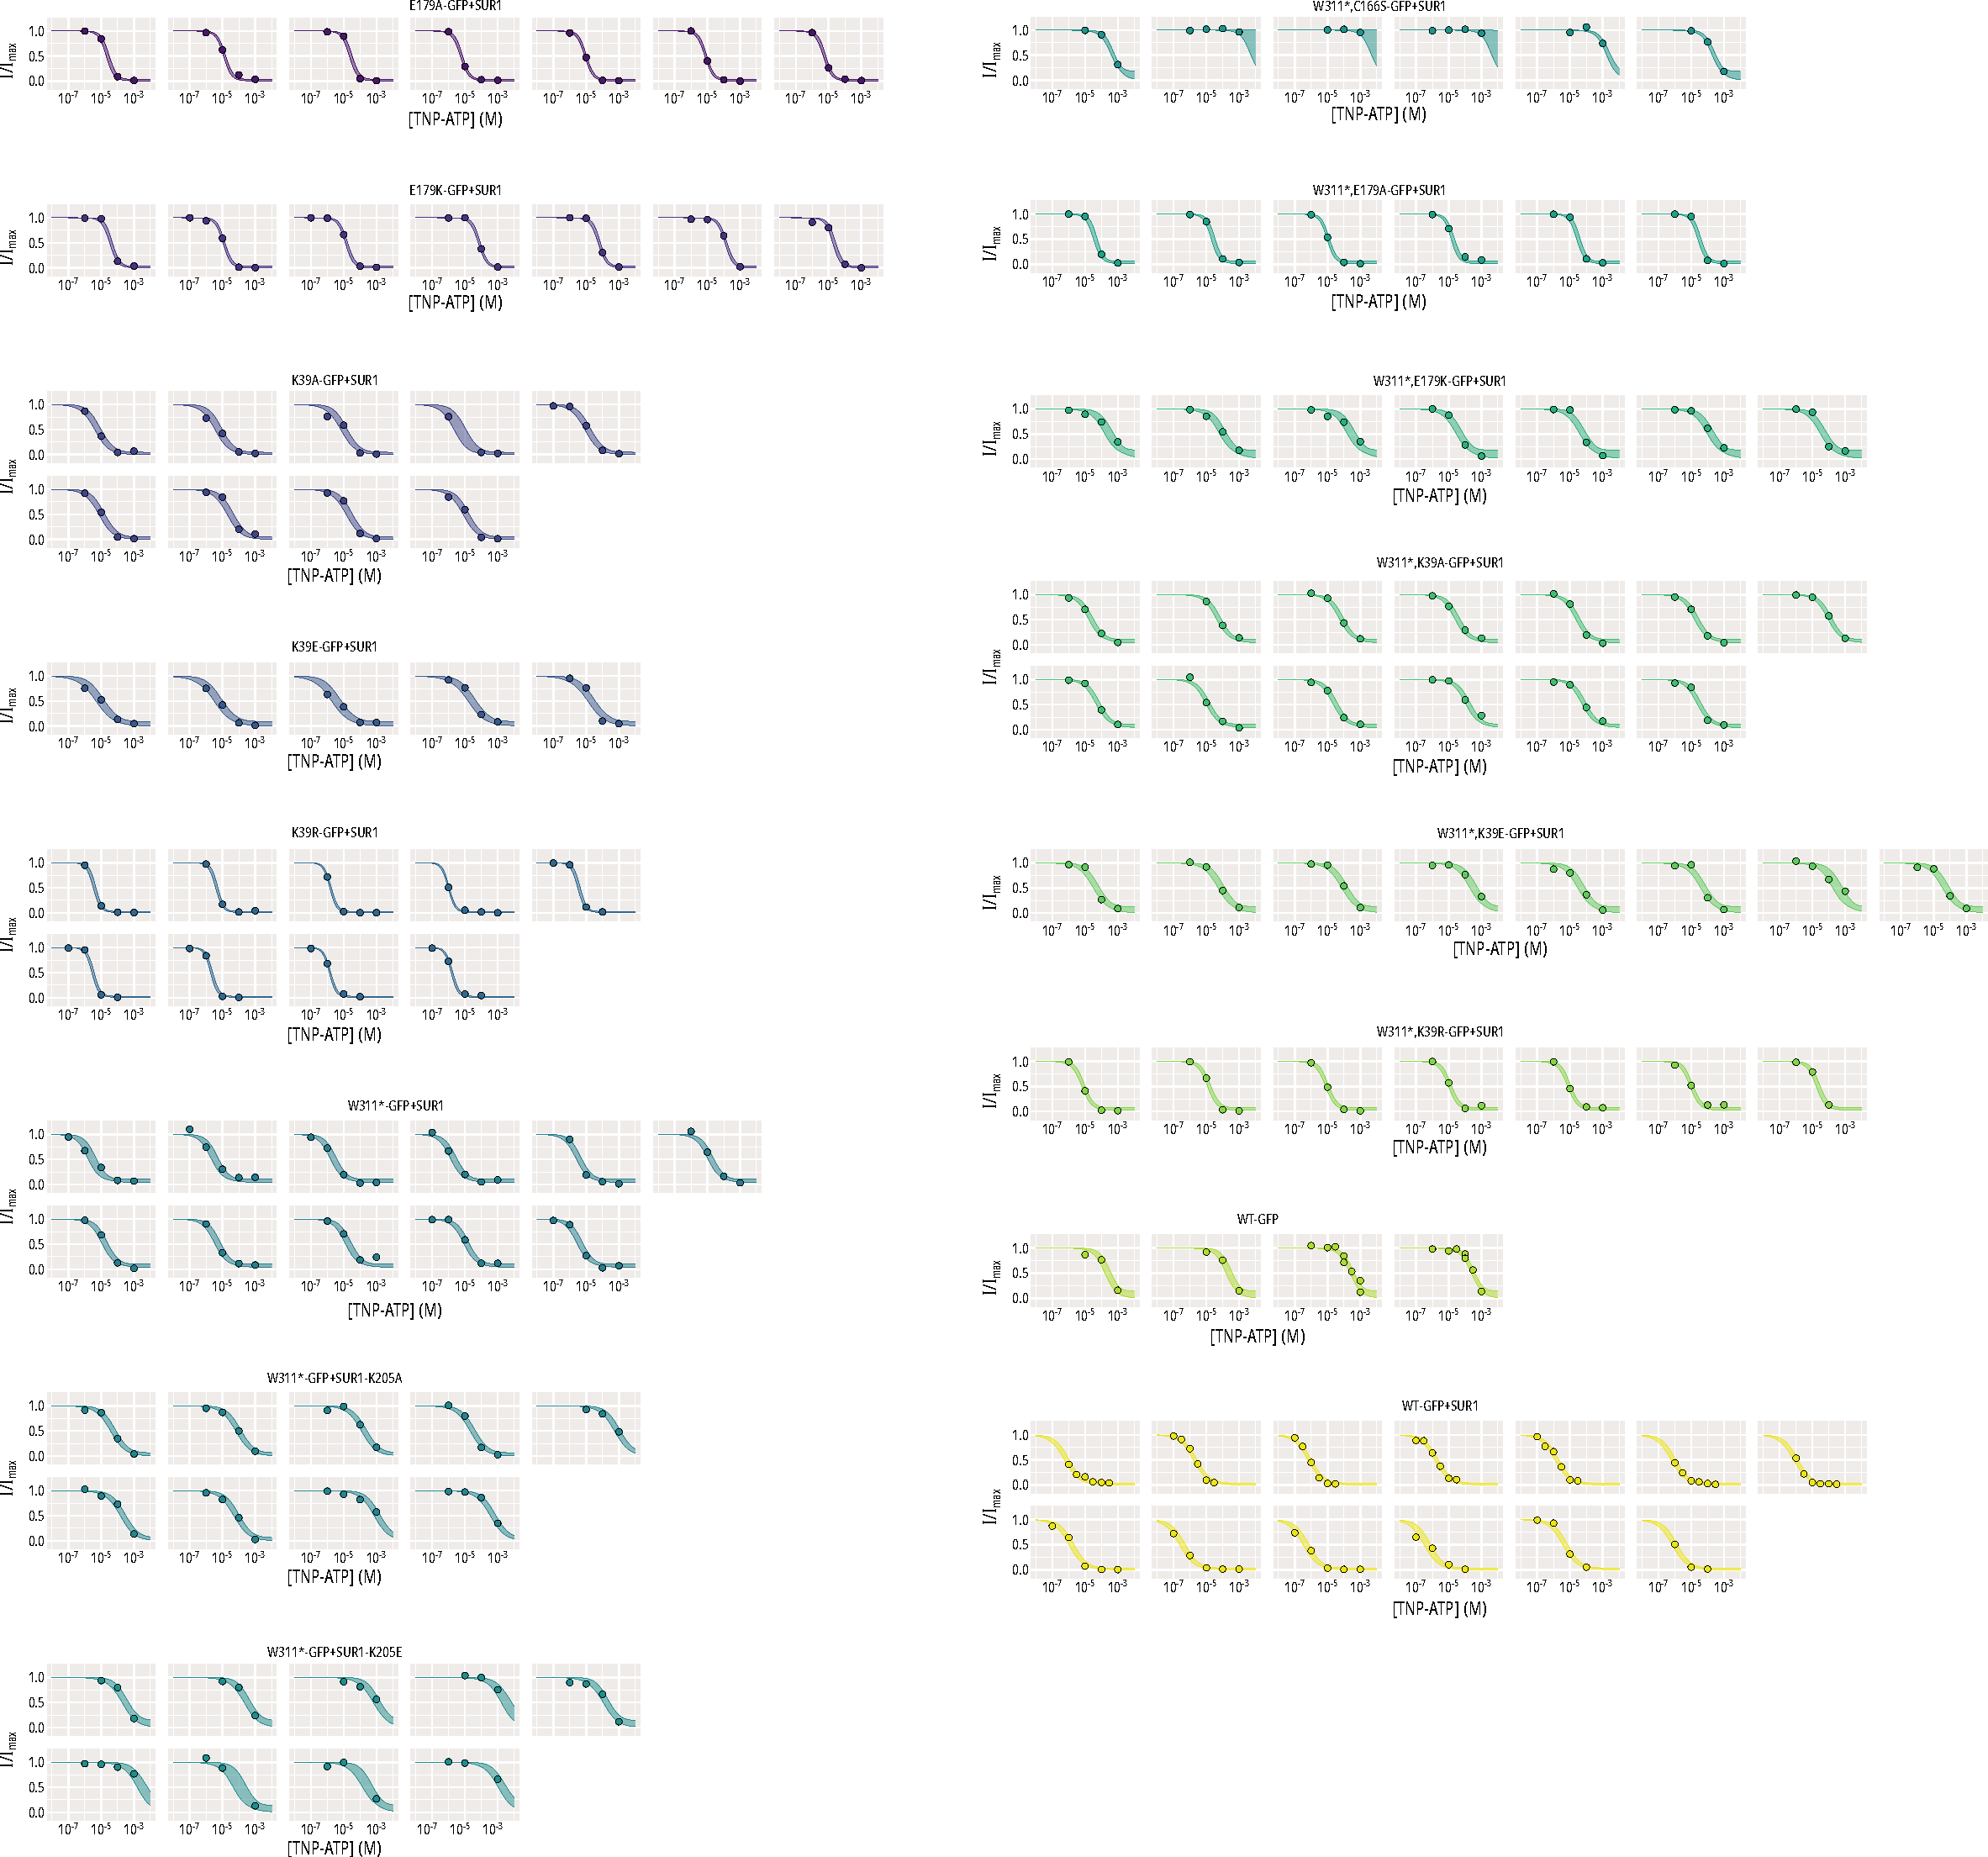
\includegraphics[width=\textwidth]{all_tnpatp_fits_2.pdf}
	\caption[TNP-ATP inhibition sample hill fits]{
	}
	\label{apxfig:tnpatp_inhib_2}
\end{figure}

\begin{figure}[h]
	\centering
	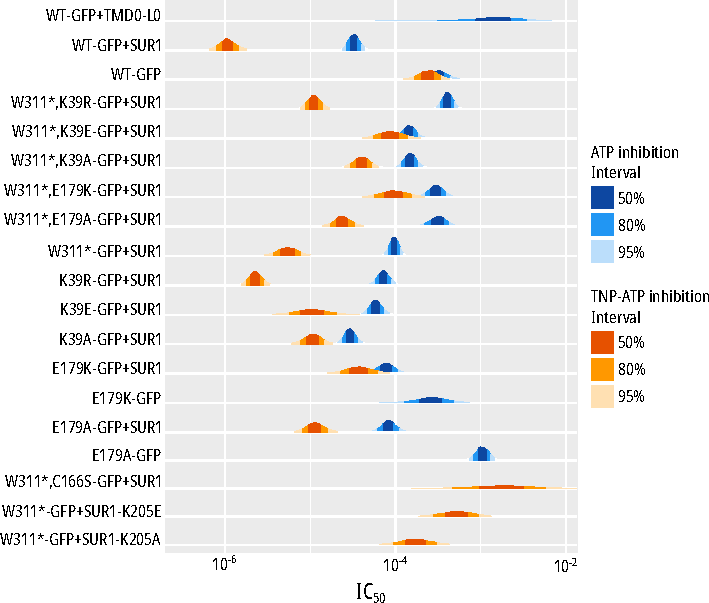
\includegraphics[width=\textwidth]{all_inhibition_params.pdf}
	\caption[Nucleotide inhibition IC\textsubscript{50} posterior distributions]{
	}
	\label{apxfig:inhib_params}
\end{figure}

\begin{figure}[h]
	\centering
	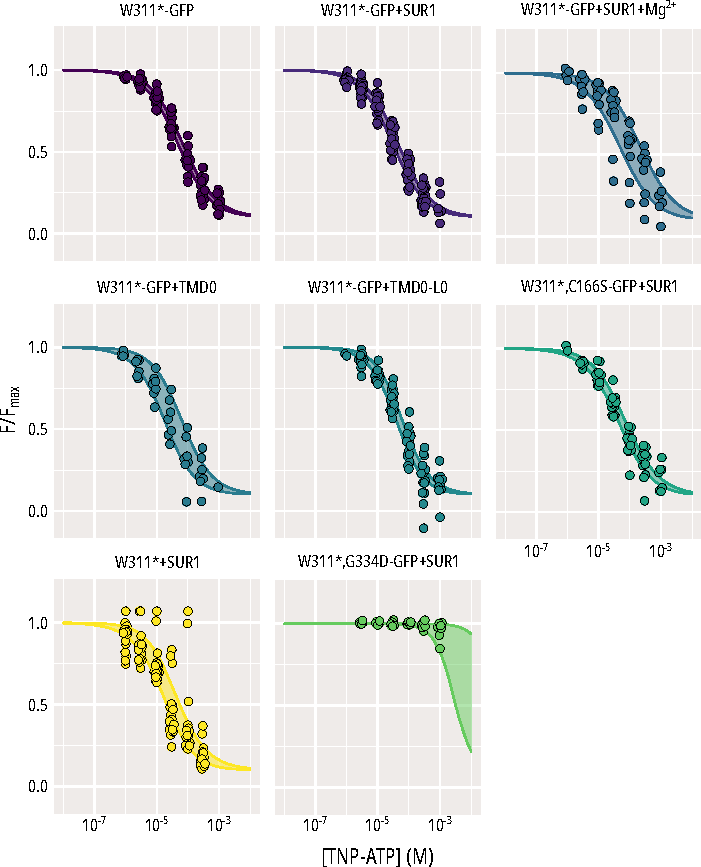
\includegraphics[width=\textwidth]{all_unroofed_fits_1.pdf}
	\caption[Unroofed membrane quenching population hill fits]{
	}
	\label{apxfig:unroofed_1}
\end{figure}

\begin{figure}[h]
	\centering
	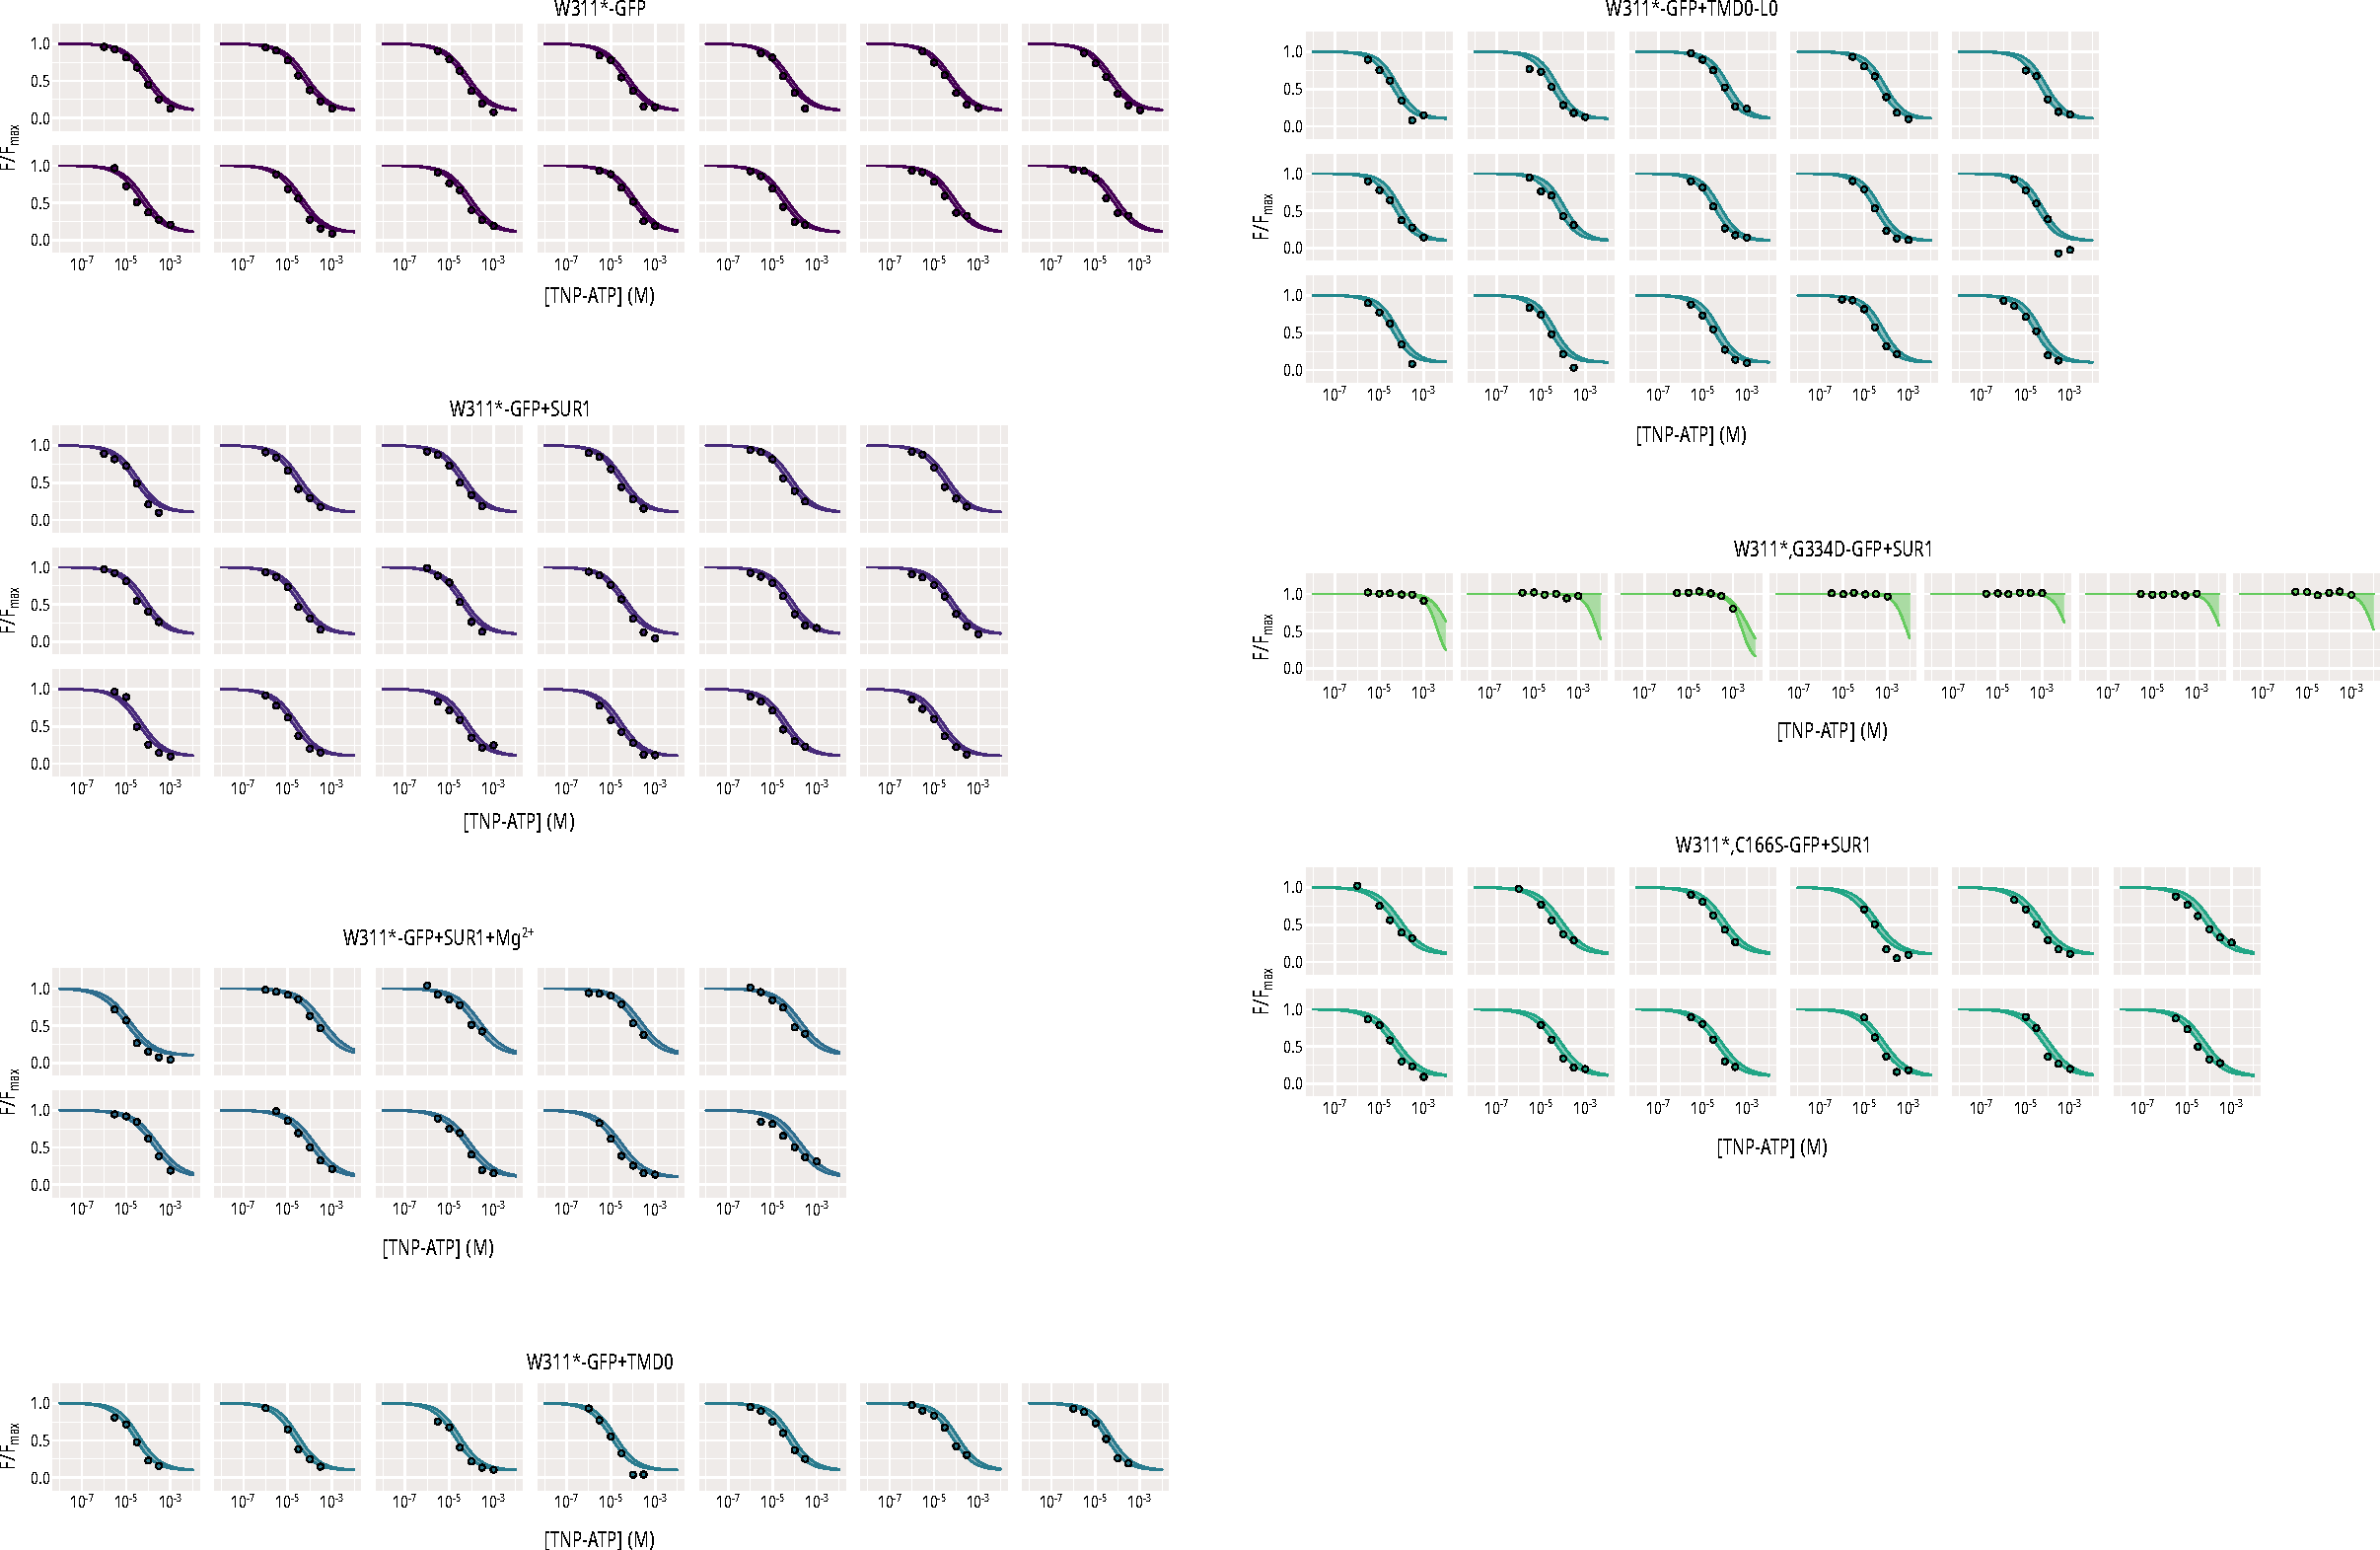
\includegraphics[width=\textwidth]{all_unroofed_fits_2.pdf}
	\caption[Unroofed membrane quenching sample hill fits]{
	}
	\label{apxfig:unroofed_2}
\end{figure}

\begin{figure}[h]
	\centering
	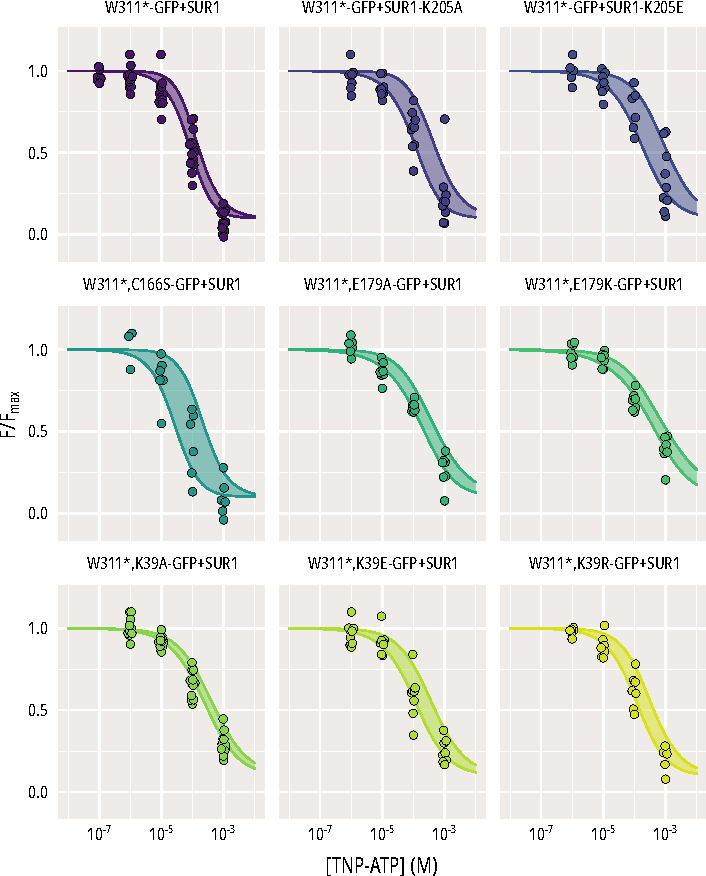
\includegraphics[width=\textwidth]{all_pcf_fits_3.pdf}
	\caption[Excised patch quenching population hill fits]{
	}
	\label{apxfig:pcf_1}
\end{figure}

\begin{figure}[h]
	\centering
	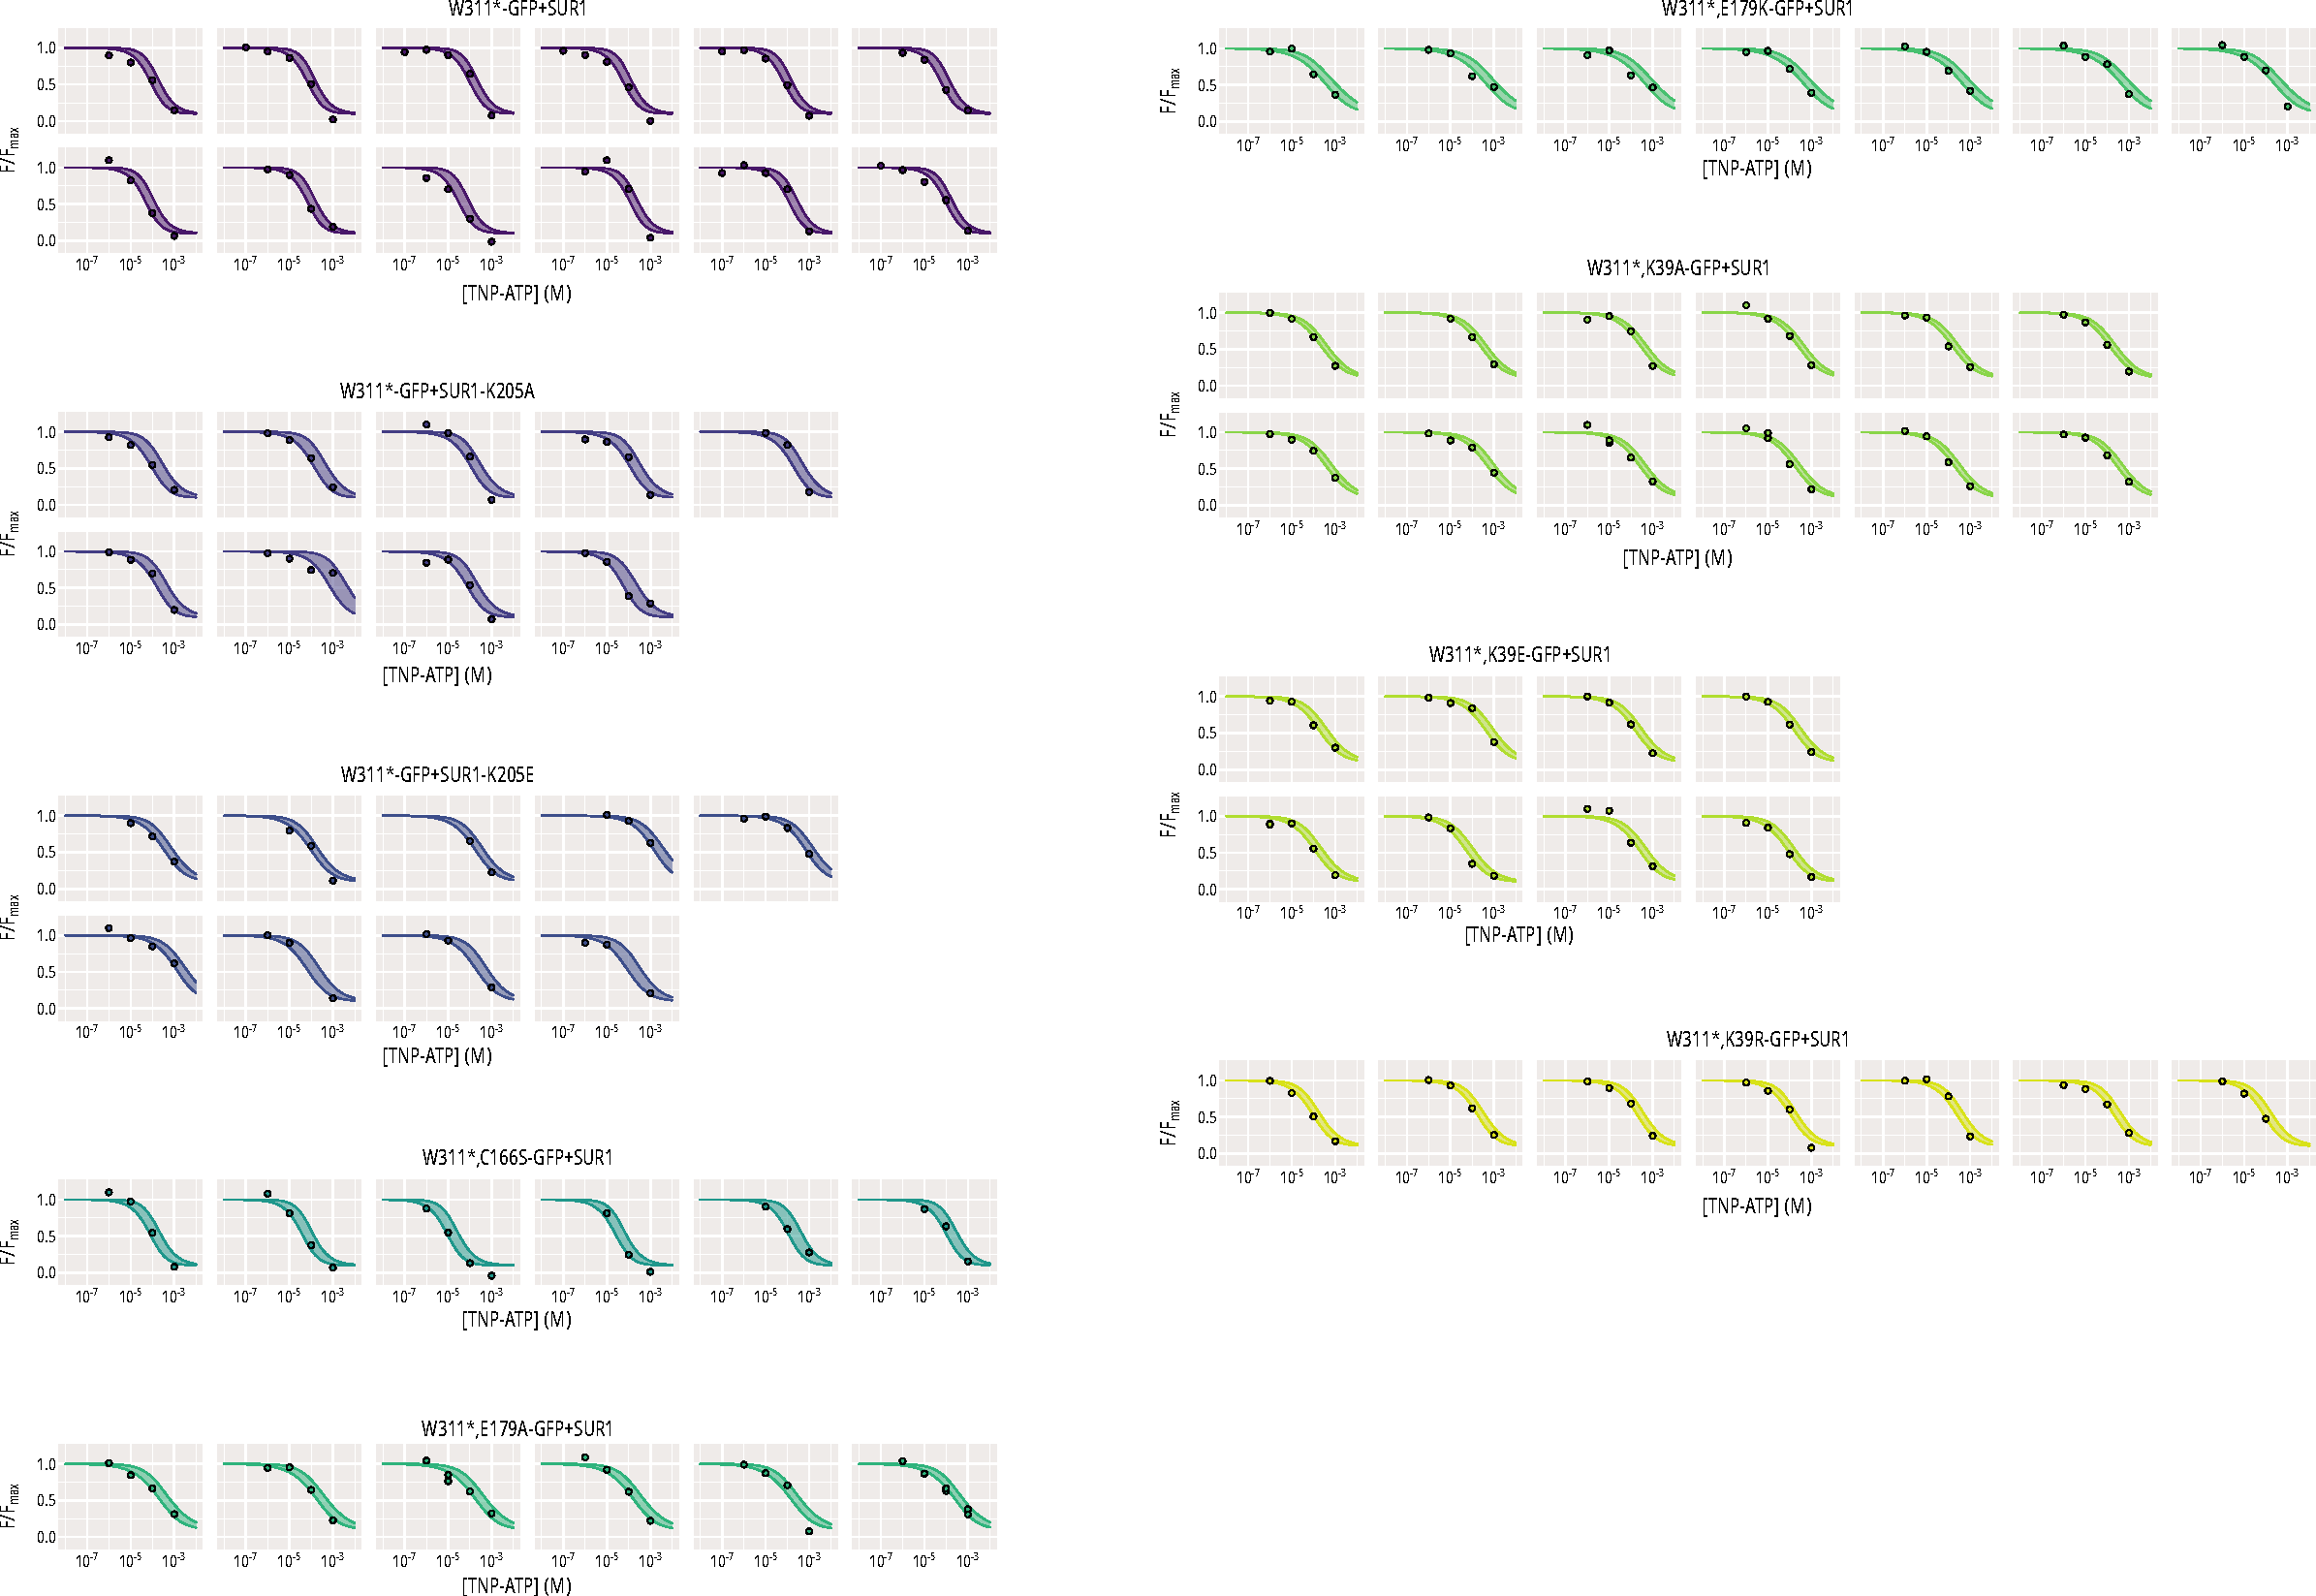
\includegraphics[width=\textwidth]{all_pcf_fits_4.pdf}
	\caption[Excised patch quenching sample hill fits]{
	}
	\label{apxfig:pcf_2}
\end{figure}

\begin{figure}[h]
	\centering
	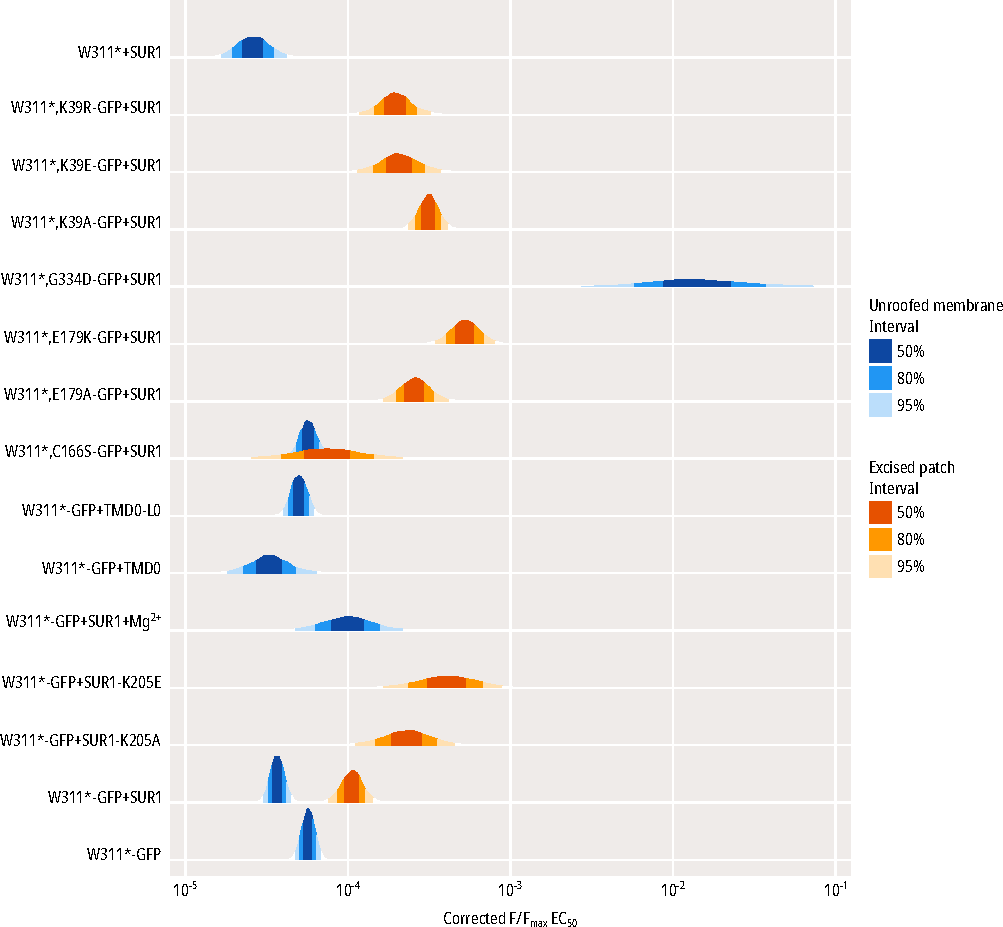
\includegraphics[width=\textwidth]{all_binding_params.pdf}
	\caption[Fluorescence quenching EC\textsubscript{50} posterior distributions]{
	}
	\label{apxfig:binding_params}
\end{figure}

\begin{figure}[h]
	\centering
	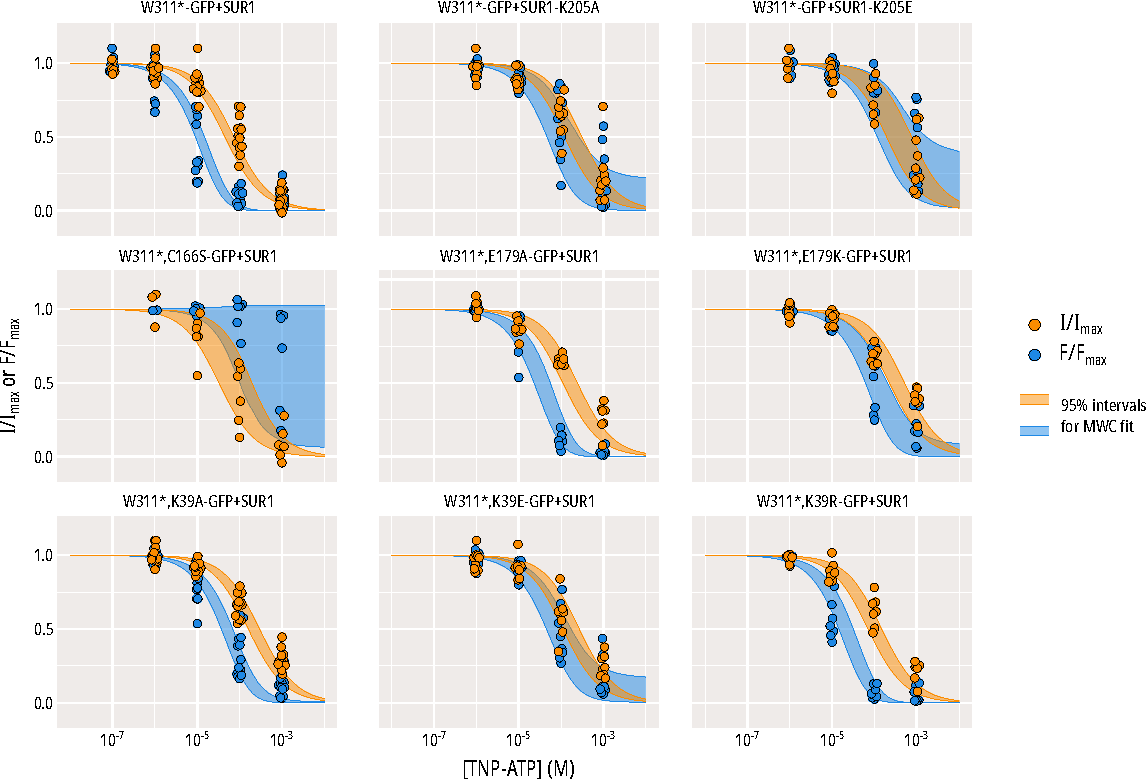
\includegraphics[width=\textwidth]{all_pcf_fits_1.pdf}
	\caption[MWC population fits]{
	}
	\label{apxfig:pcf_3}
\end{figure}

\begin{figure}[h]
	\centering
	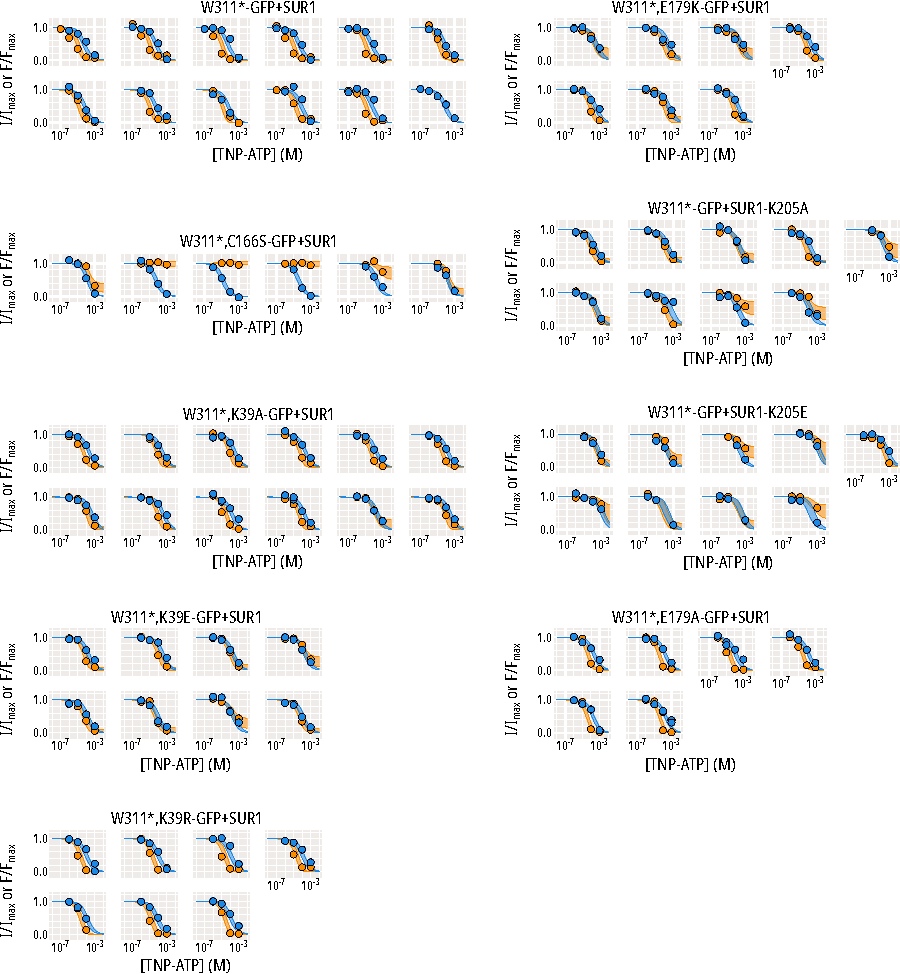
\includegraphics[width=\textwidth]{all_pcf_fits_2.pdf}
	\caption[MWC sample fits]{
	}
	\label{apxfig:pcf_4}
\end{figure}

\begin{figure}[h]
	\centering
	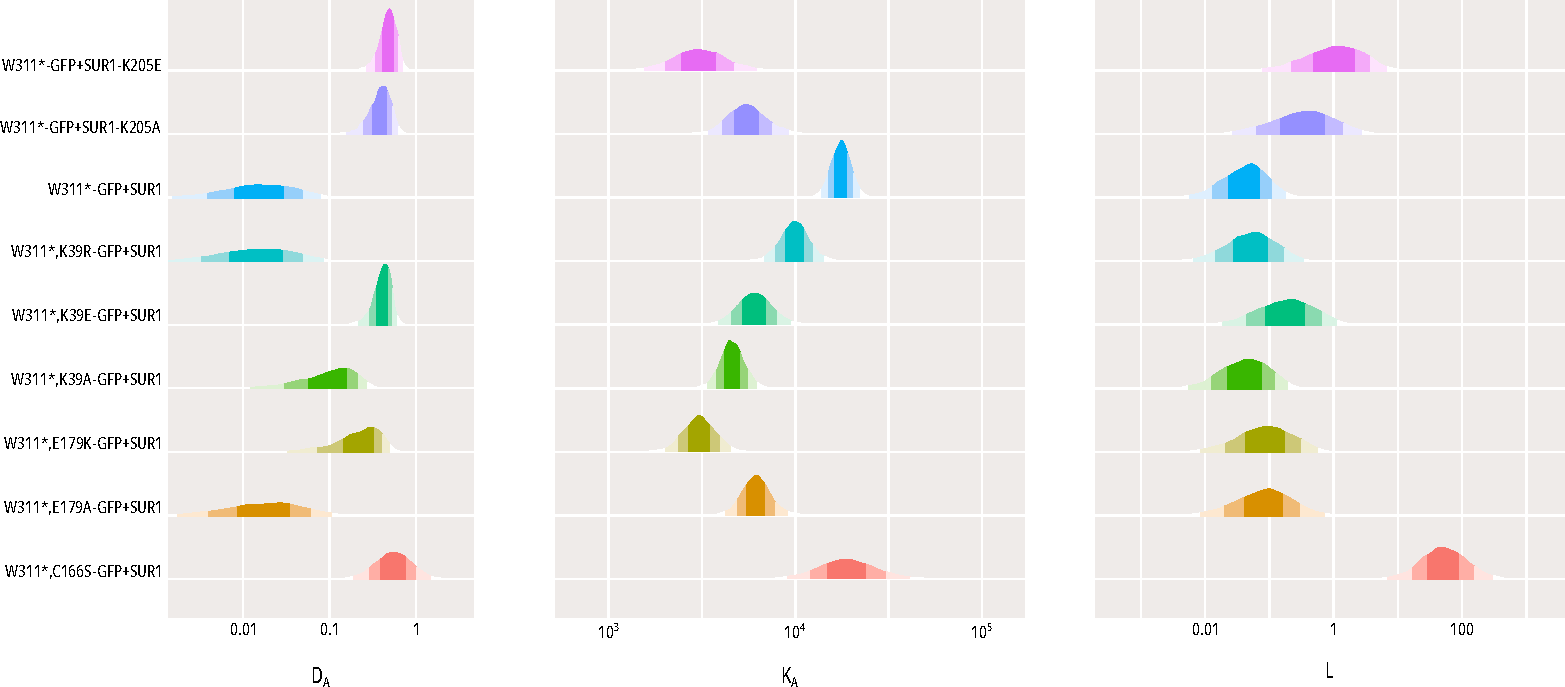
\includegraphics[width=\textwidth,angle=90,origin=c]{all_pcf_params_1.pdf}
	\caption[MWC parameter posterior distributions]{
	}
	\label{apxfig:mwc_params}
\end{figure}


%%%%% REFERENCES

% JEM: Quote for the top of references (just like a chapter quote if you're using them).  Comment to skip.
% \begin{savequote}[8cm]
% The first kind of intellectual and artistic personality belongs to the hedgehogs, the second to the foxes \dots
% \end{savequote}

\setlength{\baselineskip}{0pt} % JEM: Single-space References

{\renewcommand*\MakeUppercase[1]{#1}%
\printbibliography[heading=bibintoc,title={\bibtitle}]}


\end{document}
